\documentclass{elsarticle}\usepackage[]{graphicx}\usepackage[]{color}
% maxwidth is the original width if it is less than linewidth
% otherwise use linewidth (to make sure the graphics do not exceed the margin)
\makeatletter
\def\maxwidth{ %
  \ifdim\Gin@nat@width>\linewidth
    \linewidth
  \else
    \Gin@nat@width
  \fi
}
\makeatother

\definecolor{fgcolor}{rgb}{0.345, 0.345, 0.345}
\newcommand{\hlnum}[1]{\textcolor[rgb]{0.686,0.059,0.569}{#1}}%
\newcommand{\hlstr}[1]{\textcolor[rgb]{0.192,0.494,0.8}{#1}}%
\newcommand{\hlcom}[1]{\textcolor[rgb]{0.678,0.584,0.686}{\textit{#1}}}%
\newcommand{\hlopt}[1]{\textcolor[rgb]{0,0,0}{#1}}%
\newcommand{\hlstd}[1]{\textcolor[rgb]{0.345,0.345,0.345}{#1}}%
\newcommand{\hlkwa}[1]{\textcolor[rgb]{0.161,0.373,0.58}{\textbf{#1}}}%
\newcommand{\hlkwb}[1]{\textcolor[rgb]{0.69,0.353,0.396}{#1}}%
\newcommand{\hlkwc}[1]{\textcolor[rgb]{0.333,0.667,0.333}{#1}}%
\newcommand{\hlkwd}[1]{\textcolor[rgb]{0.737,0.353,0.396}{\textbf{#1}}}%
\let\hlipl\hlkwb

\usepackage{framed}
\makeatletter
\newenvironment{kframe}{%
 \def\at@end@of@kframe{}%
 \ifinner\ifhmode%
  \def\at@end@of@kframe{\end{minipage}}%
  \begin{minipage}{\columnwidth}%
 \fi\fi%
 \def\FrameCommand##1{\hskip\@totalleftmargin \hskip-\fboxsep
 \colorbox{shadecolor}{##1}\hskip-\fboxsep
     % There is no \\@totalrightmargin, so:
     \hskip-\linewidth \hskip-\@totalleftmargin \hskip\columnwidth}%
 \MakeFramed {\advance\hsize-\width
   \@totalleftmargin\z@ \linewidth\hsize
   \@setminipage}}%
 {\par\unskip\endMakeFramed%
 \at@end@of@kframe}
\makeatother

\definecolor{shadecolor}{rgb}{.97, .97, .97}
\definecolor{messagecolor}{rgb}{0, 0, 0}
\definecolor{warningcolor}{rgb}{1, 0, 1}
\definecolor{errorcolor}{rgb}{1, 0, 0}
\newenvironment{knitrout}{}{} % an empty environment to be redefined in TeX

\usepackage{alltt}
\usepackage[utf8]{inputenc}

\usepackage[letterpaper, margin=1.25in]{geometry}
\usepackage{amsmath}
\usepackage{enumitem}
\usepackage{caption}
\usepackage{subcaption}
\usepackage{graphicx}
\usepackage{xfrac}
\usepackage{smartdiagram}
\usepackage{booktabs}
\usepackage{float}
\usepackage{datetime}
\usepackage{lineno}

%Load in the R scripts

\graphicspath{ {figures/} }

\bibliographystyle{elsarticle-num}
\biboptions{sort&compress}
\IfFileExists{upquote.sty}{\usepackage{upquote}}{}
\begin{document}

\begin{frontmatter}


\title{Hybrid pedestrian and transit priority zoning policies in an urban street network: Evaluating network traffic flow impacts with analytical approximation}
 
%% Group authors per affiliation:
\author{Nicholas Fournier, PhD}
\address{Institute of Transportation Studies, \\
University of California, Berkeley\\
409 McLaughlin Hall, Berkeley, California 94720}


\begin{keyword}
transit priority \sep pedestrianization \sep pedestrian only zone \sep policy 
\end{keyword}

% \maketitle

\begin{abstract}
Pedestrianized zones are becoming an increasingly popular policy tool for cities seeking to improve ``walkability'', ``livability’’, and reduce congestion in the urban center by prohibiting automobiles from entering a designated zone. However, pedestrianized zones can be inappropriately implemented in locations without justifiable congestion or sufficient transit alternatives. For mixed-traffic transit (e.g., bus and light-rail streetcars), the lack of reasonable transit alternatives is an issue further compounded by the traffic congestion generated from diverted driving trips concentrated around the pedestrianized zone, inadvertently slowing down both automobile traffic and mixed-traffic transit in tandem. Alternatively, to mitigate the traffic congestion impact on transit, policy makers can also designate a ``transit priority’’ zone around the pedestrian zone, where transit is unimpeded by congestion either through transit signal priority, dedicated lanes, or both. This ensures transit provides a consistent travel alternative as congestion varies, creating a stable demand equilibrium that would otherwise be suppressed by congestion. While such a solution has been proposed in advocacy, no research has explored such a combined policy in analytical terms. This research explores the potential complementary benefits and optimal sizing of pedestrianization and transit priority zones through analytical evaluation in an idealized rectilinear city. The model is intended to provide insights regarding traffic impacts, optimal zone sizing, system capacity, and the justifiable thresholds for implementing complementary pedestrianization and transit priority zones in a city.

% \vfill

\end{abstract}

\end{frontmatter}

% \newpage

\linenumbers

\section{Introduction}
Congestion, particularly automobile congestion, is often seen as the persistent foe of economic efficiency in dense urban cities \citep{Solow1971,Solow1972,Solow1973,Anas1998,Anas1999,Wheaton1998,Rossi-Hansberg2004}. For decades, planners and engineers have sought to mitigate this endemic issue of congestion through road capacity expansion and urban density controls (i.e., land use zoning policies). However, this often comes at the demise of historic urban centers, and more recently, an affordable housing shortage due to a constrained supply of low-density single-family dwelling only zoning. In an effort to reverse this trend, planners and politicians occasionally implement pedestrian only zones as a particularly aggressive and dogmatic approach to urbanism. Pedestrian zones function by severely limiting or prohibiting automobile traffic in an area or corridor of a city, thereby enforcing walkability. 

Pedestrian zone policies have and continue to be implemented, but these experimental policies too often fail to achieve the desired results due to inadequate supporting conditions. One such condition is providing reasonable transportation alternatives (i.e., transit). Otherwise pedestrian zones could fail to attract people, or worse, end up causing more congestion as diverted routes are concentrated around the zone. Furthermore, with the bulk of transit systems operating in mixed-traffic (e.g., buses or light-rail sharing lanes with traffic), the congestion compounds the problem by further slowing transit even if transit does exist.

Another related policy is ``transit priority'', which holds a potential solution. Transit priority is often broadly defined as any policy, infrastructure, or operational strategy that gives transit priority over automobile traffic. There exists a spectrum of strategies, from signal timing to physical infrastructure, that can be used to provide some level of priority. Often, transit priority is simply a signal control strategy which provides some advantage to transit vehicles (e.g., red truncation, green extension, and progressive signal coordination), with little or no change to physical road geometry. This type of transit priority will be referred to as ``transit \emph{signal} priority''. While transit signal priority is a relatively new technology in practice, the concept itself has been experimented with since at least the 1970s \citep{Yagar1994,Yagar1993}. Although transit signal priority can provide some advantage to transit vehicles through various control strategies, effectiveness is still ultimately limited by road capacity and mixed-traffic congestion.

A more aggressive transit priority approach is to provide a physically dedicated right-of-way (e.g., bus only lane, elevated rail, or subways) which limits or restricts private vehicle traffic. In the case of bus only lanes or Bus Rapid Transit (BRT), this ensures transit vehicles are unimpeded by congestion, offering rail-like service reliability at a fraction of the cost. Unfortunately, transit priority generally comes at high cost (e.g., rail) or the loss of valuable road space and capacity (e.g., bus only lanes taking a traffic or parking lane) and is seldom politically popular \cite{Nash2003}. However, where the political will exists to implement pedestrian zones, transit priority is a modest extension but holds enormous complementary benefits and is ideally suited to mitigating the possible shortcomings of pedestrianization policies. Moreover, by ensuring that transit operates unimpeded, it provides a demand stabilizing effect. As automobile congestion and travel time rise, a reliable transit alternative becomes a more attractive mode choice, creating a stable demand equilibrium and preventing demand from being suppressed by high travel times due to congestion \cite{Wardrop1952,Gonzales2013,Tabuchi1993,Vickrey1969}. 

This notion of suppressed demand is also important when considering other policy levers for travel demand management, such as pricing (e.g., transit fares, tolls, congestion pricing, parking pricing, etc.). Imposing pricing policies offers an effective means of controlling travel demand and moving towards a more effective equilibrium point without major infrastructure investment \citep{Li2014, Lou2010, Huang2002, Wang2004, Yang1997, Zheng2012, Huang2000, Gonzales2012, Danielis2002}. However, without any reasonable travel alternatives, such as transit, demand will simply be suppressed. This may alleviate congestion, but does little to support economic activity or personal mobility and accessibility.

In an effort to preserve or revitalize urban centers and reduce congestion, pedestrian zones and transit priority are two increasingly popular planning policy tools. However, neither pedestrianization nor transit priority are new concepts, urban planners and community activists have been advocating for more ``walkable'' \citep{Brambilla1977,Pushkarev1975,Engwicht2007} and ``transit oriented'' \citep{Owen1972,Walbridge1977} urban environments for decades. This paper will, however, not delve into vast philosophy of urban theory and planning existentialism. The purpose is more narrowly focused on travel time reduction through the complementary benefits of pedestrianized zones and transit priority. However, it is important to equip the reader with the background understanding of ``urbanism'' to explain why cities might seek to reverse their automobile dependence. 

While there have been numerous studies and books published highlighting the potential social, environmental, and economic benefits of walkability and pedestrian-centric design, these studies often lack an objective and quantitative evaluation to justify their claims. Conversely, there have been a multitude of technologically driven engineering research on transit signal priority \cite{Skabardonis2000,Dion2002,Dion2004} and optimization \cite{Stevanovic2008,Mesbah2011,Ma2013}, but are too narrowly focused site-specific performance to realize the greater systemic benefits if broadly implemented in a city, let alone with pedestrianization \citep{Mesbah2008,Sanchez2008,Wang2012}. This research aims to bridge the gap between planning and engineering by modeling the combined effect of pedestrianized and transit priority zones in an analytical model of an idealized city in order to explore the possible outcomes. 

To many ``traditional'' traffic engineers, pedestrianization and transit priority may appear as radical, inefficient, and directly in opposition to their efforts to provide an efficient transportation system for the modern economy. But it is important to consider the broader contextual motivation of such policies; that is, to create urban environments for people in cities, not their automobiles. Traffic engineers are not necessarily wrong, many pedestrian oriented concepts are loose abstract philosophies, lacking tangible and objective solutions for the modern world. This paper seeks to help remedy this by providing a mathematical analysis of a pedestrianized zone surrounded by transit priority. The problem is simplified for an idealized city with a rectilinear grid street network in order to explore a range of outcomes. The purpose of this paper is to not only provide a model, but to demonstrate the complementary benefits of such policies in a generalized and objective form.

\subsection{Modeling philosophies}
Among academics, there is often a muted tension between idealized analytical modeling approaches and empirical models. Analytical models are theoretical approaches using continuous mathematical approximations based on physical and geometric properties, often applied to represent static traffic equilibrium or transit network operations and explore hypothetical outcomes \citep{Newell1973,Badia2017,Badia2014,Chen2015,Daganzo2010,Holroyd1967,Sivakumaran2012,Vaughan1987}. While analytical approaches offer elegant solutions, more complex problems are not easily solved, such as traffic assignment and dyanmic mode-choice, requiring stochastic or deterministic numeric solutions \citep{Dial1996,Watling2006,Chen2010,DePalma1983,Daganzo1977}. Prior to the proliferation of high-powered computation over the last few decades, classical analytical models largely dominated. Since then, the field has given way to more data driven discrete choice, simulation models, and more recently, artificial intelligence capable of high-resolution predictions far beyond simplistic analytical models \citep{Ben-Akiva1981,Ben-Akiva1985,Ben-Akiva1986,McFadden1981,Train1978,Ziemke2016}. 

Analytical models are often rightfully criticized as being overly simplified and hyper-idealized cases with little or no practical application outside of academic text. While true that simulation's precision offers abundant practical applications (e.g., travel demand models and system optimization), they are often immensely sophisticated ``black-box'' estimations, rely on past data, and too frequently validated against other simulated results. This obscures any broad functional systemic relationships that might exist and limits simulation results only to where sufficient explanatory data exists; and not with, for example, untested pedestrianized and transit priority zones. Analytical models in contrast, focus primarily on those functional relationships, helping shed broader insight for policy that can then later be refined through simulation. 

The following analytical model is not meant to provide high-resolution results, nor is it meant to provide a grand unifying mathematical function. It is merely intended to demonstrate in quantitative terms, the potential complementary benefits of pedestrianized zones surrounded by transit priority. The goal is that a simplified, objective, and unbiased model might help dissolve some of the opinions and misguided advocacy that might lead to an impractical or inappropriate policy decisions. Of course, this model is hyper-idealized, only measures travel time, and does not account for the multitude of other social and economic factors beyond basic commuter behavior. It is possible that if the results were implemented in broad strokes, as was done with the automobile oriented boom of the 20\textsuperscript{th} century, there would most likely be numerous unexpected negative side effects. The results should not be taken as cause to radically rebuild, but to help better understand the potential benefits that pedestrianization and transit priority have in increasing system capacity and reducing travel times. 


\section{Concept}
Consider an idealized city of dimension $R$ with rectilinear street network with spacing $d$, as shown in Figure~\ref{fig:gridcity}. Demand can be defined by two types of trip patterns, baseline uniform travel demand across the city and monocentric trips to and from the city center. The cumulative effect is increased congestion in the city center. To make the city center more attractive, ``livable'', and ``walkable'', policy makers designated a square pedestrianized zone of size $\gamma$ in the city center, allowing only pedestrians, bicycles, and transit vehicles. The pedestrianized zone forces drivers entering the center of the city to park at the perimeter and walk, possibly increasing travel time. This increased travel time potential makes transit more attractive if transit can still enter the pedestrianized zone. However, the pedestrianized zone forces drivers to divert routes around the zone, increasing traffic density and congestion as a result. To mitigate the traffic congestion impact on transit (e.g., buses and streetcars/trams), policy makers also designated a ``transit priority'' area of dimension $\tau$, around the pedestrian zone, where transit is unimpeded by congestion either through transit signal priority, dedicated right-of-way (e.g., bus only lane, elevated track, or subways), or both
. 

\begin{figure}[H]
     \centering
     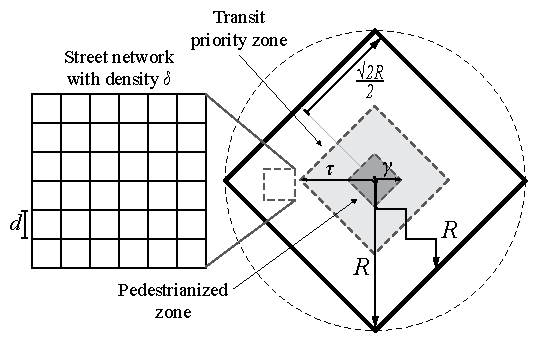
\includegraphics[width=0.5\textwidth]{diagram_pedtransit_grid_city}
     \caption{Rectilinear city with pedestrianized zone}
     \label{fig:gridcity}
\end{figure}

Typically, transit priority is not conceptualized as a zone. In practice, transit priority is typically implemented along designated radial corridors leading towards the city center. However, at a macroscopic regional scale, transit priority generally falls within a central region of a city where traffic congestion is severe enough to justifies transit priority. Thus, in this conceptualization it is not necessarily that every street within the transit priority zone has transit priority, but the transit corridors in the zone are unimpeded by transit.

\subsection{Mode choice}
Mode choice in this model is fundamentally a binary choice between between driving and transit. However, if their destination is located within the pedestrianized zone, they can either take transit for the entire trip or drive to the perimeter and walk the remaining distance within the pedestrianized zone. The decision criterion is assumed to be based on travel time. Although travel time is a major factor affecting mode choice, it is important to note that in reality it is only one among many factors (e.g., safety, comfort, accessibility, cargo, etc.) \citep{DeGruyter2019,Currie2020}. For simplicity, this model assumes that mode choice depends entirely on travel time, meaning that travelers choose whichever mode provides the shortest travel time. However, future extensions of this model could partially account for biases or other ``utilities'' by weighting the travel times associated with each mode. 

Assuming that driving and mixed-traffic transit are delayed by automobile congestion but transit priority and pedestrians are not, then it may be possible to manipulate travel time and demand through complementary pedestrian and transit priority zoning policies, described in Figure~\ref{fig:gridcity}. Congestion in the city center may be eliminated by imposing a pedestrianized zone, forcing drivers to walk the remaining distance. This may forcibly eliminate congestion in the city center, but sizing of the pedestrian zone is critical as any reduction in congestion delay may be quickly outweighed by perimeter road congestion and the additional time spent walking if the zone is too large. For transit priority, its stable travel time becomes more attractive as driving demand and congestion increase. However, assuming transit cannot exceed the speed of automobiles (i.e., there is a speed limit), then there is no benefit to providing transit priority beyond where congestion exists in the city. Conversely, if no transit priority exists, then transit will always be slower than driving due to stops and dwell time, offering little incentive for drivers to change modes. Based on these assumptions, a model can be formulated to minimize travel time by manipulating the size a pedestrianized zone and transit priority zone, finding an optimal size of both. 

\subsection{Objective}
The objective of this conceptual model is to minimize average total travel time for travelers in the city by determining the optimal pedestrian only and transit priority zone sizes. While both the pedestrian only and transit priority zone ultimately contribute to the primary objective of reducing average total travel time, they both have their own individual objectives and constraints. The pedestrian zone on its own has the objective of preventing traffic flow from exceeding capacity in the city center. The transit priority zone is then subsequently implemented to mitigate any increased travel time due to excess walking distance or traffic generated by the pedestrianized zone. The goal in this paper is to reduce the two problems such that they share the same parameters and can be evaluated in single unified objective function accounting for both policies simultaneously. 
There are three basic components necessary to build and evaluate the conceptual model:

\begin{enumerate}
    \item Travel demand -- the number of trips and their flow direction. 
    \item Travel distance -- the average trip distance per mode.
    \item Travel time -- the average travel time per mode which depends upon demand-based congestion.
\end{enumerate}

From these three components, the average total travel time can then be calculated and evaluated. The following subsections will discuss the necessary components in further detail.

\subsection{Travel demand}
Demand is generated in the city area in units of $\frac{trips}{dist^2 \cdot time}$, and can be simplified into two types:

\begin{itemize}
    \item uniform baseline travel across the network, $\lambda_b$, and 
    \item monocentric travel demand going to and from the centroid of the city, $\lambda_c$. 
\end{itemize}

Average trip flow can be calculated as the product of trip demand and average trip length, divided by the amount of roadway infrastructure available to carry these trips, yielding trip flow in units of $\frac{trips}{lane \cdot time}$. Thus, the baseline traffic flows (see Figure~\ref{fig:basetrips}) associated with average trip length\footnote{
	The average baseline distance, $l_b$ can be calculated from the expected Manhattan distance distributed across a unit square, $E(D) = \iint\iint \frac{1}{4}\left(|x_1 - x_2| + |y_1 - y_2| \right ) dy_2 dx_2 dy_1 dx_1$ with the limits of $-R \leq x_1 \leq R$, $|x_1|-1 \leq y_1 \leq 1-|x_1|$, $-1 \leq x_2 \leq 1$, and $|x_1|-1 \leq y_2 \leq 1-|x_1|$. Since $|x_1 + x_2|$ and $|y_1 + y_2|$ are identical, it can be simplified to $2\int_{-1}^{1} \int_{-1}^{1} |x_1 - x_2|(1-|x_1|)(1-|x_2|)dx_2 dx_1$, which evaluates to $\frac{14}{15}$ as proportional to any size $R$, thus $l_b = \frac{14}{15}R$. The average monocentric Manhattan distance, $l_c$, to the center of the square is equivalent to the Euclidean distance to the center in a circle of size $R$, thus the average expected distance is $l_c = \frac{2}{3}R$ \cite{Stone1991}. The overall average travel distance is then $l = \frac{R(14\lambda_b + 10\lambda_c)}{15(\lambda_b + \lambda_c)}$.
}, $l_b$, generate $q_b = \frac{\lambda_b l_b}{\delta}$ flow across the network, where $\delta$ is the roadway network density\footnote{
The calculation for network density can be derived as the total roadway length $2n(n+1)d$, divided by total area $nd^2$; both of which can be expressed as a function of the number of city blocks $n$, and the street spacing dimension $d$. The relationship between $\delta$ and $d$ is linearly constant, yielding $\delta = \frac{2}{d}$.
} in units of $\frac{lane \cdot dist}{dist^2}$. There is then the additional traffic flow associated with monocentric trips to and from the center that varies with the distance from the center (see Figure~\ref{fig:monotrips}). Consider a square of infinitesimal perimeter width $dr$, at distance $r$ from the center, the total demand for trips crossing this square is $2\lambda_c (R^2 - r^2)$. The trips generated by this demand then travel a distance $dr$ across the square using the available road infrastructure of $4\sqrt{2}r\delta$.

\begin{figure}[H]
	\centering
	%\hfill
	\begin{subfigure}[b]{0.35\textwidth}
		\centering
		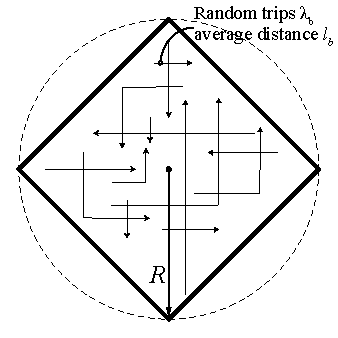
\includegraphics[width=\textwidth]{diagram_trips_base}
		\caption{Baseline trips across city, $q_b$}
		\label{fig:basetrips}
	\end{subfigure}
	%\hfill
	\begin{subfigure}[b]{0.35\textwidth}
		\centering
		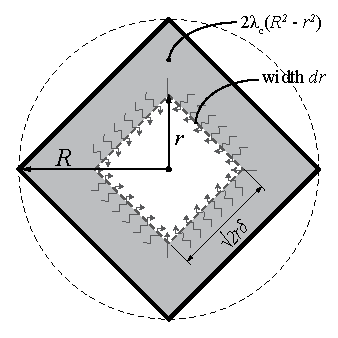
\includegraphics[width=\textwidth]{diagram_trips_mono}
		\caption{Monocentric trips at distance $r$, $q_m$}
		\label{fig:monotrips}
	\end{subfigure}
%	\hfill
	\caption{Baseline and monocentric trip diagram}
\end{figure}


The average monocentric flow through the network at a point with a distance $r$ from the city center is then $q_m(r) = \frac{2\lambda_c \left(R^2 - r^2\right)}{4\sqrt{2}\delta r}$. The combined flow at distance $r$ from the city center is then the combined sum, calculated as:

\begin{equation}
    q_a(r) = \frac{14R\lambda_b}{15\delta} + \frac{\lambda_c}{2\sqrt{2}\delta r} \left(R^2 - r^2 \right)
    \label{eq:flowacross}
\end{equation}

\noindent The pedestrianized zone will cause some trips to be diverted around the pedestrian zone along a square perimeter zone created by the ``pinch points'' at the corners. Assuming travelers choose the shortest route, but will choose an available equidistant route to avoid congestion, trips in the city can be categorized into four distinct types (see Figure~\ref{fig:diverted}):

\begin{enumerate}
	\item Unimodal routes entirely within the pedestrianized zone that are unaffected by congestion, 
	\item Bimodal routes taking vehicles to perimeter of pedestrianized zone to park nearest the destination and the remaining radial distance is traveled on foot,
	\item Unimodal routes entirely outside the pedestrianized zone that can avoid congestion created by the zone, and
	\item Unimodal routes that would have passed through the center, whose shortest paths are now diverted to the ``pinch points'' created by the pedestrianized zone vertically and horizontally.
\end{enumerate}

\begin{figure}[H]
     \centering
     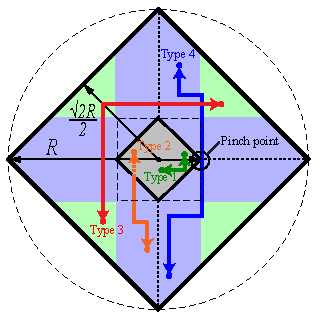
\includegraphics[width=0.4\textwidth]{diagram_diverted_routes}
     \caption{Example diverted route types}
     \label{fig:diverted}
\end{figure}

\noindent In a rectilinear grid, multiple equidistant paths exist that can be used to avoid congestion. Trip types 2 and 3 can avoid traveling along the pinch point perimeter by taking an earlier or later turn without increasing distance. However, trip type 4 cannot avoid the pinch point perimeter unless extra turning movements or a longer path is taken. While a longer route can and will be chosen in reality, the worst case is assumed that travelers will choose the shortest path and face congestion at these pinch point perimeter roads. To determine the trip flow along this perimeter, the shaded areas in Figure~\ref{fig:diverted} denote the contributing demand area for each trip type. The expected trip flow (vehicle-distance/time) on the perimeter road is the product of three values: the number of trips originating in the critical city half between $\gamma$ and R, $\lambda_b (R^2 - \gamma^2)$; the probability that a trip destination falls within the trip category, $\frac{\gamma(R-\gamma)}{R^2}$; and the expected distance per trip on the pinch point perimeter road, $2\gamma$. Dividing the total in $\frac{trips \cdot dist}{time}$ by the length of the perimeter traversed\footnote{It is conservatively assumed that travelers traverse the entire perimeter edge to avoid extra turning movements.}, $2\gamma$, provides the critical flow in $\frac{trips}{time}$ on the perimeter road:

\begin{equation}
	q_p(\gamma) = \frac{\lambda_b \gamma (R-\gamma) (R^2 - \gamma^2)}{R^2}
    \label{eq:perimflow}
\end{equation}

The trip demand flow density across the network at distance $r$ from the city center, from the function in Equation~\eqref{eq:flowacross}, possesses the form shown in Figure~\ref{fig:flowacross}. As the distance from the city increases, traffic decreases. When traffic near the center exceeds capacity, one might consider simply pedestrianizing the city center out to the point where capacity is no longer exceeded. However, as more trips are diverted around the perimeter zone, traffic congestion on the perimeter road can increase as the zone size increases. The trip demand flow around the perimeter of the pedestrian zone, from Equation~\eqref{eq:perimflow}, possesses a parabolic-like shape with a long-tailed right side, shown in Figure~\ref{fig:perimflow}.

An interesting note is that the long-tailed parabolic-like form is unique to rectilinear grids. A ring-radial street network yields a half parabola-like form centered at the origin so that a non-zero pedestrianized zone starts with the maximum traffic, then rapidly improving at an accelerating rate \citep{Fournier2019}. The reason for this is not immediately apparent, but makes intuitive sense when considering possible route alternatives in each network structure.

As a pedestrianized zone in a rectilinear grid increases in size, it causes a larger number of trips to be diverted around the perimeter, increasing perimeter road traffic. However, once the pedestrianized zone becomes so large, a majority of trips are entirely contained within the pedestrianized zone, causing perimeter road traffic to decrease. Somewhat counter-intuitively in a ring-radial city, the traffic congestion is worst for the smallest non-zero pedestrianized zone. This is because, unlike in a rectilinear grid, there are no equidistant alternative routes around the perimeter road, making the perimeter route the shortest route. In reality it is more likely that traffic congestion in the ring-radial network will find some equilibrium flow distributed across the network, rather than concentrate along one route. However, urban road networks are seldom ever a geometrically perfect rectilinear grid or ring-radial structure, and may even be some combination of the two. 

In either case, the pedestrianized zone may eliminate congestion in the city center, but would greatly increase travel time by walking. An appropriate policy might try to find a balance between where the city center is pedestrianized enough to reduce congestion in the center, but not too much to create perimeter road congestion.

\begin{figure}[H]
     \centering
     \hfill
     \begin{subfigure}[b]{0.45\textwidth}
         \centering
         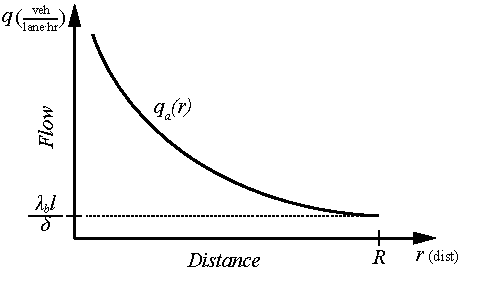
\includegraphics[width=\textwidth]{diagram_flow_across}
         \caption{Trip demand flow at point $r$ distance from the city center}
         \label{fig:flowacross}
     \end{subfigure}
     \hfill
     \begin{subfigure}[b]{0.45\textwidth}
         \centering
         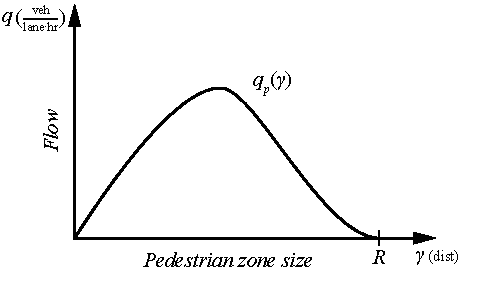
\includegraphics[width=\textwidth]{diagram_flow_perim}
         \caption{Trip demand flow on perimeter road of pedestrian zone size $\gamma$}
         \label{fig:perimflow}
     \end{subfigure}
     \hfill
     \caption{Trip demand flow}
\end{figure}

\subsection{Travel distance}
To determine the travel time, the total average distance traveled must be calculated for each travel mode. The average travel distance for driving, pedestrians, and transit are described in the following sub-sections.

\subsubsection{Average driving distance}
The driving distance is the average driving distance for baseline trips ($\frac{14}{15}(R-\gamma)\times\frac{\lambda_b}{\lambda_b + \lambda_c}$) and monocentric trips ($\frac{2}{3}(R-\gamma)\times\frac{\lambda_c}{\lambda_b + \lambda_c}$) outside of the pedestrian zone, multiplied by the proportion of respective trip demand. The combined function can be simplified to

    \begin{equation}
    l_D = \frac{(R-\gamma)(14\lambda_b + 10\lambda_c)}{15(\lambda_b + \lambda_c)}
    \end{equation}

\subsubsection{Average pedestrian distance}
Pedestrian trips are also generated by the baseline demand (b) and the monocentric central demand (c). Let $D_{ij}$ be demand amount and $l_{ij}$ be the average walking distance covered in each case $ij$ where $i$ is trip types $\{1,2\}$ and $j$ is demand type $\{b,c\}$. The total distance covered within the pedestrianized zone $l_P$ is then:
    
    \begin{equation}
         l_P = \frac{\sum\limits_{i,j} D_{ij}l_{ij} }{\sum\limits_{i,j} D_{ij}}
    \end{equation}
    
    where: 
    \begin{itemize}
        \item $D_{1b} = 2 \lambda_b \gamma^2 \times \frac{\gamma^2}{R^2}$ : Total baseline demand trips originating in pedestrian zone by the proportion ending in the pedestrian zone.
        \item $D_{2b} = 4 \lambda_b (R^2 - \gamma^2) \times \frac{\gamma^2}{R^2}$ : Total baseline demand trips originating inside and ending outside the pedestrian zone, and vice versa. Both cases equal $2\lambda_b (R^2 - \gamma^2) \times \frac{\gamma^2}{R^2}$.
        \item $D_{1c} = 2 \lambda_c \gamma^2$ : Total monocentric trips originating inside the pedestrian zone.
        \item $D_{2c} = 2 \lambda_c (R^2 - \gamma^2)$ : Total monocentric trips originating outside the pedestrian zone.
        \item $l_{1b} = \frac{14}{15}\gamma$ : Average distance of baseline trips that originate and end in the pedestrian zone.
        \item $l_{2b} = \gamma$ : Average distance of baseline trips that originate from the pedestrian zone perimeter (i.e., the point where traveler changes mode to walk) to some uniformly distributed destination in the zone.
        \item $l_{1c} = \frac{2}{3}\gamma$ : Average distance of monocentric trips that originate and end in the pedestrian zone.
        \item $l_{2c} = \gamma$ : Average distance of monocentric trips that originate from the pedestrian zone perimeter to the city center.
    \end{itemize}
    
    The combined function then becomes:
    
    \begin{equation}
    l_{P}=\frac{-32\lambda_{b}\gamma^{5}+\left(60\lambda_{b}+5\lambda_{c}\right)R^{2}\gamma^{3}+15R^{4}\lambda_{c}\gamma}{15\left(4\lambda_{b}R^{2}\gamma^{2}-2\lambda_{b}\gamma^{4}+2R^{4}\lambda_{c}\right)}
    \end{equation}

\subsubsection{Average transit distance}
    Transit distance must be separated by the portion traveled in transit priority and in mixed traffic to calculate the appropriate travel time:
    
    \begin{itemize}
        \item In mixed traffic it is the average distance traveled outside the priority zone:
        
        \begin{equation}
            l_{TM} = \frac{(R-\tau)(14\lambda_b + 10\lambda_c)}{15(\lambda_b + \lambda_c)}
        \end{equation}
            
        \item In transit priority it is the average distance traveled inside the priority zone:
        
        \begin{equation}
            l_{TP} = \frac{\tau (14\lambda_b + 10\lambda_c)}{15(\lambda_b + \lambda_c)}
        \end{equation}
        
    \end{itemize}


\subsection{Travel time}
The average total travel time is calculated using the respective travel time functions for each mode type and demand split: 

\begin{equation}
	\bar{t}_{total}(\gamma,\tau) = \Phi_D(\tau) \times \bigg( \bar{t}_D(\gamma) + \bar{t}_P(\gamma) \bigg) + \bigg(1-\Phi_D(\tau) \bigg) \times \bigg( \bar{t}_{TP}(\tau) + \bar{t}_{TM}(\tau) \bigg)
\end{equation}

\noindent where $\bar{t}_{total}(\gamma,\tau)$ is the average total travel time, $\bar{t}_D(\gamma)$ is the average driving travel time, $\bar{t}_P(\gamma)$ is average travel time within the pedestrianized zone, $\bar{t}_{TP}(\tau)$ is the average transit priority travel time, $\bar{t}_{TM}(\tau)$ is the average mixed-traffic transit travel time, and $\Phi_D(\tau)$ is the proportion of trips driven by car. These travel times are calculated using the respective travel demand and distances described in previous sections. However, in addition to this travel time, delay due to congestion will be experienced for driving and mixed-traffic transit. This congested travel time will be discussed in the following subsections.

\subsubsection{Traffic flow}
Congested travel time (i.e., driving and mixed traffic transit) depends upon the state of traffic flow through the network. Traffic flow through the network can be characterized by the macroscopic fundamental diagram (see Figure~\ref{fig:mfd}) as a function of trip demand density \citep{Daganzo2008, Geroliminis2008, Liu2016, Haddad2014}. A travel time function (see Figure~\ref{fig:traveltime}) then depends upon the state of traffic flow through the network as being either ``uncongested'' (solid line) or ``congested'' (dashed line) in Figures~\ref{fig:mfd} and~\ref{fig:traveltime}.\footnote{Literature has also classified these two states as ``congestion'' and ``hypercongestion'', where any traffic density affecting traffic speed (i.e., any density $k>0$) is considered ``congested'' and when capacity is exceeded (i.e., when density $k \geq k_c$) it is ``hypercongested'' \citep{Gonzales2015,Small2003}.}

\begin{figure}[H]
     \centering
     \hfill
     \begin{subfigure}[b]{0.45\textwidth}
         \centering
\begin{knitrout}
\definecolor{shadecolor}{rgb}{0.969, 0.969, 0.969}\color{fgcolor}
\includegraphics[width=\maxwidth]{figure/flowdensity-1} 
\end{knitrout}
         \caption{Macroscopic fundamental diagram}
         \label{fig:mfd}
     \end{subfigure}
     \hfill
     \begin{subfigure}[b]{0.45\textwidth}
         \centering
\begin{knitrout}
\definecolor{shadecolor}{rgb}{0.969, 0.969, 0.969}\color{fgcolor}
\includegraphics[width=\maxwidth]{figure/timeflow-1} 
\end{knitrout}
         \caption{Travel time cost function}
         \label{fig:traveltime}
     \end{subfigure}
     \hfill
     \caption{Macroscopic fundamental diagram and travel time cost function}
\end{figure}

Although a variety of more refined macroscopic models have been developed, many are often very sophisticated and require additional calibration parameters, or possess abrupt transitions that can create anomalies in analytical results. Two common classical models that require no additional calibration parameters are Greenshields' \citep{Greenshields1935} parabolic function and Daganzo's \citep{Daganzo1997} bi-linear model. Greenshields' seminal function is elegantly simple, but symmetric parabolic shape has since been proven a poor fit in reality, particularly when critical density, $k_c$, is exceeded. Daganzo's model in contrast provides a very simple parsimonious model with an asymmetric form, but its linearity assumes a constant free-flow speed until it abruptly transitions at critical density. The constant free-flow speed not only ignores minor delay caused by gradual slowing of traffic as density increases, but causes an abrupt transition that can cause erroneous results with the sudden jump. 

Assuming for this case a parabolic function represents the uncongested portion of the flow-density relationship, an expression for the ``uncongested'' solid line portion of Figure~\ref{fig:mfd} can be written as:

\begin{equation}
    q(k) = q_{c}\frac{k\left(2k_{c}-k\right)}{k_{c}^{2}}
\end{equation}

\noindent where $k_c$ is the density at capacity, and $q_c$ is the flow at capacity. In order to determine travel time, density as a function of flow $k(q)$ can be solved as a quadratic:

\begin{equation}
    k(q) = k_c \left(1 - \sqrt{1- \frac{q}{q_c}} \right)
    \label{eq:densityparabolic}
\end{equation}

\noindent However, a problem in calculating travel time using the macroscopic fundamental diagram is its concave form which results in a backward bending travel time function once trip demand exceeds capacity \citep{Gonzales2015}. From this flow-density, a piece-wise monotonic cost function for travel time, as shown in Figure~\ref{fig:traveltime}, can then be defined as:

\begin{equation}\
	t(q) = 
	\begin{cases}
		q  <  q_{c} : & l \frac{k(q)}{q} \\
		q \ge q_{c} : & t_c \left(\frac{q}{q_c}\right)^{20} = l \frac{k_c}{q_c} \left(\frac{q}{q_c}\right)^{20}
	\end{cases}
\end{equation}

\noindent where $t(q)$ is travel time for flow $q$, $k(q)$ is traffic density for flow $q$, $l$ is link length, $q_c$ is link capacity, and $t_c = l\frac{k_c}{q_c}$ is the travel time at capacity. The congested portion for travel time can be simply modeled as a sufficiently steep monotonically increasing function. To avoid an abrupt transition from the uncongested portion, a very high exponent of 20 was chosen to closely match the parabolic function's trajectory without being perfectly vertical. This provides a smooth transition from parabolic to exponential. The average travel time in traffic $\bar{t}$, can be determined from the average travel distance $\bar{l}$, divided by average speed $\bar{v}$:

\begin{equation}
    \bar{t} = \frac{\bar{l}}{\bar{v}} = \bar{l}~\frac{k\left(\bar{q_a}\right)}{\bar{q_a}}
\end{equation}

\noindent which can be analytically determined from the macroscopic fundamental diagram as a function of average flow across the network $\bar{q}_a$, as experienced by travelers from their trips between the pedestrian zone $\gamma$, and the city limit $R$:

\begin{align}
    \bar{q}_a & = \frac{1}{R-\gamma}\int_\gamma^R q(\gamma) d\gamma \notag\\
    \bar{q}_a & = \frac{14R\lambda_{b}}{15\delta} +  \frac{\lambda_{c}}{8\delta (R - \gamma)} \left[ 2R^{2} ln \left( \frac{R}{\gamma}\right) + \gamma^{2} - R^{2}\right]
\end{align}

\noindent which can then be used to determine the average travel time in traffic.

\subsubsection{Transit}
Transit travel time is conditional upon whether it operates in a transit priority zone (e.g., dedicated lane or right-of-way) or in mixed-traffic (e.g., city bus). In transit priority it is assumed there is no other source of delay other than delay due to stopping, which can be calculated from the average lost time from stopping, $t_s$, and the stop spacing, $s$. In mixed traffic the transit travel time is this stopping delay plus delay from congestion. These travel times can be calculated as:

\begin{subequations}
\begin{align}
    t_{TP} & = \frac{l}{v_{m}} + \frac{l}{s}t_s & \text{with transit priority} \\
    t_{TM}(q) & = l\frac{k(q)}{q} + \frac{l}{s}t_s   & \text{without transit priority when}~q < q_c\\
    t_{TM}(q) & = l\frac{k_c}{q_c} \left(\frac{q}{q_c}\right)^{20} + \frac{l}{s}t_s & \text{without transit priority when}~q \geq q_c
\end{align}
\label{eq:ttfunc}
\end{subequations}

\noindent where $v_m$ is the maximum cruising speed of transit unimpeded by traffic. The stop time is essentially the lost time inclusive of acceleration, deceleration and dwell time. The travel time of transit in mixed-traffic will then always be higher than driving an automobile. A similar observation was also found by Geroliminis et al. \citep{Geroliminis2014} using a bi-modal three-dimensional macroscopic fundamental diagram. In this model, the travel times will eventually converge as traffic conditions reach jam flow. Conversely, transit priority provides a constant travel time which will be initially slower than driving in uncongested traffic conditions, but will eventually reach a traffic flow point $q_T$, where the travel time of transit with priority exceeds driving (see Figure~\ref{fig:transittraveltime}).

\begin{figure}[H]
    \centering
    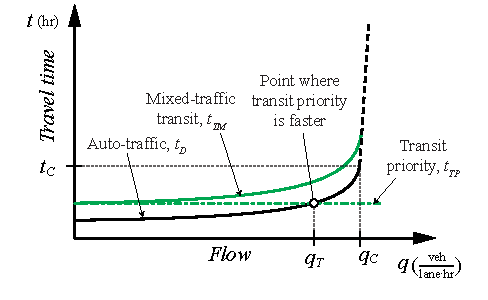
\includegraphics[width=0.5\textwidth]{diagram_transit_traveltime}
    \caption{Driving and transit travel time}
    \label{fig:transittraveltime}
\end{figure}

The critical transit priority traffic flow point $q_T$, is found where transit priority travel time $t_{TP}$ intersects driving travel time $t_D$. Since travel time is a piece-wise function, it depends on whether the transit priority travel time $t_{TP}$, exceeds the driving travel time at roadway capacity $t_c$. Although it is unlikely that transit priority travel time will exceed this point, the condition is provided nonetheless. To determine when this occurs, a simple ratio can be taken, $\sfrac{t_{TP}}{t_c}$. The critical transit priority traffic flow point then depends on whether $\sfrac{t_{TP}}{t_c}$ is greater than or less than 1:

\begin{subequations}
\begin{align}
    q_T & = \frac{2k_{c}}{T} - \frac{k_{c}^{2}}{q_{c}T^{2}} & \text{for}~ \sfrac{t_{TP}}{t_c} < 1 \\
    q_T & = q_{c}\left(\frac{q_{c}}{k_{c}}T\right)^{\frac{1}{20}} & \text{for}~ \sfrac{t_{TP}}{t_c} \geq 1 \\
    \end{align}
    \text{where: }
    \begin{align}
    T & = \frac{1}{v_{m}} + \frac{t_{s}}{s}  \notag \\
    \sfrac{t_{TP}}{t_c} & = \frac{q_c}{k_c} \left( \frac{1}{v_m} + \frac{t_s}{s}  \right) \notag
    \end{align}
\end{subequations}

For simplicity, it is assumed that transit priority does not affect driving in this model. In reality it is possible that transit and transit priority may affect driving conditions. For example, if a driving lane is taken from cars to create a dedicated bus lane or if bus traffic is high enough to congest overall traffic. However, it is possible that ``transit priority'' could be designed or constructed to minimize or avoid any impact on driving conditions. For example, some signalization strategies that gives transit priority with minimal traffic impacts, or a separate transit right-of-way was added that does not take away from driving lanes. An example of this would be and elevated track or underground subway, a form of ``transit priority'' that has existed for centuries. Nonetheless, it should be stated that transit priority can impact driving conditions but is not accounted for in this model.

As stated, many assumptions are used to make this model tractable and parsimonious. However, it may be possible to better account for the effects of mixed-traffic transit using more sophisticated models. There exists a growing body of research that extends the macroscopic fundamental diagram to include an additional dimension for transit vehicles \citep{Zheng2013,Geroliminis2014,Loder2017}. These models begin to dissect the vehicle fleet in the traffic flow, so that the relative proportion of buses and automobiles can account for the different, yet combined effect of a mixed-traffic flow. This multidimensional stratification enables details for the respective modes to be better understood, and even optimized using one unified model, the macroscopic fundamental diagram \citep{Zheng2016,Zheng2016a}. However, the added complexity of a multi-dimensional model makes the objective in this problem, to determine the optimal pedestrian and transit zone sizes, far more difficult to solve. Future work could investigate this area of research.

\section{Zone sizing}
There are two zones that require sizing, the pedestrian only zone and the transit priority zone. The two zones have varying goals but which can work simultaneously to improve travel flow across the city holistically. The pedestrian zone is concerned with preventing traffic flow from exceeding roadway network capacity in the center. However, the zone cannot be too large as to cause perimeter road traffic to exceed capacity or to cause travel times to increase due to walking. Thus, transit priority is then concerned with mitigating excess congestion around the pedestrianized zone by providing a stable travel alternative. The sizing of the pedestrianized zone and transit priority zone are described in more detail in the following two subsections.

\subsection{Pedestrian zone sizing}
Assuming policy makers wish to select a pedestrian zone size that does not cause trip demand to exceed roadway capacity, two constraints must be considered. First, the zone must be large enough to prevent traffic flow across the network from exceeding capacity $q_a(\gamma) < q_c$. Second, it must also be small enough to prevent perimeter traffic flow from also exceeding capacity $q_p(\gamma) < q_c$. Thus, a feasible pedestrian zone size can exist anywhere between $q_a(\gamma) \leq q_c \geq q_p(\gamma)$, as shown Figure~\ref{fig:flowcombo}.

 \begin{figure}[H]
     \centering
     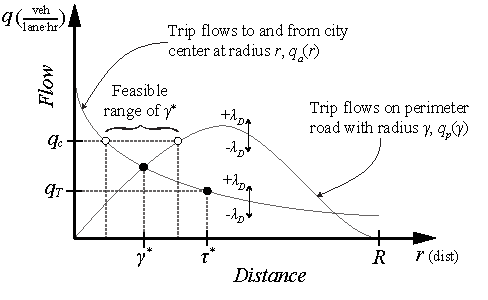
\includegraphics[width=0.5\textwidth]{diagram_flow_combo}
     \caption{Pedestrian and transit priority zone size}
     \label{fig:flowcombo}
 \end{figure}

However, this three point intersection of $q_a$, $q_p$, and $q_c$ (as shown in Figure~\ref{fig:flowcombo}) is not guaranteed since the functions are independently affected by the two demand types (i.e., monocentric and baseline demand). The first constraint depends on the monocentric demand $\lambda_c$ generating flow to and from the center, $q_a$. The second constraint depends on baseline demand $\lambda_b$ generating flow around the perimeter road, $q_p$. This means that if one trip demand type is so low $q_a$ or $q_p$ never exceeds $q_c$ in the positive space (i.e., when $q$ and $r \geq 0$), then that constraint does not exist. This creates three possible cases:

\begin{enumerate}[label=(\alph*)]
    \item If both functions intersect with capacity, then $q_a(\gamma^*) \leq q_c \geq q_p(\gamma^*)$ \label{case:mutdom}
    \item If $\lambda_c \ll \lambda_b$ so only $q_a$ intersects with capacity, then $q_a(\gamma^*) \geq q_c$ \label{case:monodom}
    \item If $\lambda_c \gg \lambda_b$ so only $q_p$ intersects with capacity, then $q_p(\gamma^*) \geq q_c$ \label{case:basedom}
\end{enumerate}

While any point in these ranges are feasible, for mathematical convenience, the intersection points can be used to calculate pedestrian zone size. In case \ref{case:monodom} and \ref{case:basedom}, this makes finding the solution relatively simple by setting the respective functions equal to roadway capacity $q_c$. This ensures that the size is at least exactly small or large enough to meet capacity by selecting the minimum or maximum pedestrian zone size. However, in case \ref{case:mutdom} where both functions meet capacity, either point could be used. As a ``compromise'', the intersection of the two flow functions could be used, ensuring both constraints are satisfied while the least possible traffic flow condition in either function is used. However, setting $q_a = q_p$ to find the intersection point results in a quintic function (polynomial to the 5\textsuperscript{th} power):

\begin{equation}\footnotesize
f(\gamma) = \lambda_{b}\left(\frac{1}{R^{2}}\gamma^{5}-\frac{1}{R}\gamma^{4}-\gamma^{3}\right)+\left(\lambda_{b}R+\frac{\lambda_{c}}{4\delta}\right)\gamma^{2}-\frac{14R\lambda_{b}}{15\delta}\gamma-\frac{\lambda_{c}R^{2}}{4\delta}
\end{equation}

\noindent yielding multiple points where the function is equal to zero (see Figure~\ref{fig:optimalped}) and cannot be easily solved analytically.

\begin{figure}[H]
     \centering
     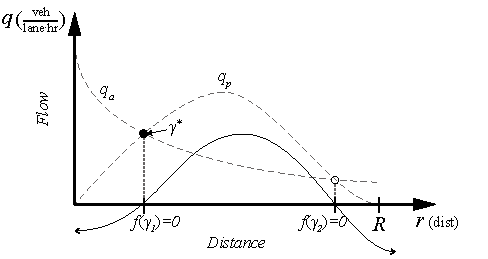
\includegraphics[width=0.5\textwidth]{diagram_optimalped}
     \caption{Quintic function for optimal compromise pedestrian zone size, $f(\gamma)$}
     \label{fig:optimalped}
\end{figure}

Given that the pedestrian zone size must exist between $0 \leq \gamma \leq R$, the number of feasible solutions in the domain is reduced, allowing for an pedestrian zone dimension $\gamma^*$ to be found numerically. Since two intersection points between $q_a$ and $q_p$ exist, the minimum of the two provides the desired optimal compromise, $\gamma^*$:

\begin{align}\small
\gamma^* &\Leftarrow \text{min} \left[ f(\gamma_1) = 0, f(\gamma_2) = 0 \right]\\
\text{s.t.} & ~ 0 \leq \gamma\leq R  \notag 
\end{align}

To summarize, the pedestrianized zone essentially functions by ``chopping off'' traffic flow before it exceeds capacity. The relative size of this zone is largely dependent on demand, increasing as monocentric demand increases, and decreasing as baseline demand increases. However, as the pedestrian zone size increases, average travel time also increase due to increasing walking distance and whatever unmitigated traffic remains outside of the zone. This section has addressed finding an appropriate pedestrian zone size, but has not yet considered traffic induced delay. Transit priority can then be enacted to reduce travel time and offset some of this unmitigated traffic demand, essentially providing a stable travel time alternative to driving.

\subsection{Transit priority zone size}
The necessary transit priority zone size can be determined using the critical transit priority traffic flow $q_T$ (see Figure~\ref{fig:transittraveltime}). This value can be used in combination with network flow at distance $r$ in Equation~\eqref{eq:flowacross} to determine the necessary transit priority zone size, $\tau^*$, when $q_T = q_a$. The reason that $q_a$ is used, and not $q_p$, is because transit priority is concerned with traffic congestion experienced in the network outside of the pedestrian zone, not just at the perimeter. Solving then for $q_T = q_a$ yields a quadratic function, but assuming a non-negative value for the optimal transit zone size, it can be solved for analytically:

\begin{align}
    \tau^*(\Phi_D) & = \frac{56 \Phi_D \lambda_{b}-60\delta q_{T} +\sqrt{\left(56 \Phi_D \lambda_{b}-60\delta q_{T}\right)^{2} + (30 \Phi_D \lambda_{c} R)^2 }}{30 \Phi_D \lambda_{c}}\\
    \text{s.t.} & ~ \tau^* \geq 0 \nonumber
\end{align}

\noindent where the proportion of driving trips, $\Phi_D$, is introduced to scale driving demand to account for mode choice between driving and transit. Unlike the optimal pedestrian zone, which us unaffected by changes in driving demand, the optimal transit priority zone size will depend on driving demand. This is because, assuming $\lambda_c$ and $\lambda_b$ are affected by mode choice equally, both $q_a$ and $q_p$ shift vertically, keeping $\gamma^*$ constant (See Figure~\ref{fig:flowcombo}). 

Although the proportion $\Phi_D$ may be modeled as a discrete choice probability, this requires travel time as an input, making optimal $\tau$ difficult to find as it creates a dynamic problem. Fortunately, since since $\gamma^*$ remains constant relative to demand, the necessary proportion of driving demand $\Phi_D$ to achieve $q_a = q_T$ (see Figure~\ref{fig:optimalped}) can be determined directly as a function of $\tau$:

\begin{equation}
    \Phi_D(\tau) = \frac {-60\delta \tau q_{T}}{15\tau^{2}\lambda_{c} - 56 \tau \lambda_{b} - 15\lambda_{c}R^{2}}
\end{equation}

\noindent With the proportion of drivers, $\Phi_D$, determined as a function of transit priority zone size, $\tau$; the travel time function in Equation~\eqref{eq:ttfunc} is now dependent on only the pedestrian and transit priority zone sizes of $\gamma$ and $\tau$, respectively.

\subsubsection{Relationship of demand and transit priority zone size}
It should be very clearly stated here that this $\Phi_D$ is \emph{not} mode choice per se, but merely the proportion of driving demand so that driving travel time is equal to transit priority travel time for the given $\tau$. The inferred assumption here is that mode choice depends solely on travel time and is equally substitutable, meaning that travelers do not have a preference for driving over transit. This, of course, is a gross over assumption, but for simplicity this analysis will carry on with this assumption. However, future models might calibrate by assuming some proportionally weighted travel time cost to account for mode preference. For example, transit travel costs $w$ more than driving, e.g., $t_{transit} = w t_{drive}$. This would have the effect of increasing $q_T$ and $\tau$, meaning that travelers are willing to tolerate more time in traffic before they step foot on a bus.

An interesting caveat to this function is that unlike true mode choice, the function for the proportion of driving demand, $\Phi_D$, can go beyond 0 and 1. If it exceeds 1 this means that more than 100\% of demand must drive in order to achieve $q_a = q_T$ for a transit priority zone size of $\tau$. This occurs when traffic conditions do not reach the level necessary to justify transit priority at $\tau$, and a smaller $\tau$ must be chosen to increase driving demand. This may seem like an erroneous outcome of the model, but is actually a useful way to determine if a transit priority zone of size $\tau$ is appropriate. If the transit priority zone size is already the smallest it can be (i.e., $\tau = \gamma$ or $\tau = 0$), then this means that transit priority is never justifiable because there is not enough overall travel demand in the city itself for $q_a = q_T$. Conversely, the function can also yield a negative value if $\tau < 0$. However, this would require a negative demand or negative transit priority zone.

This $\Phi_D$ function can be used to explore transit priority applicability. When total demand in the city varies, it alters the steepness of the driving proportion function, $\Phi_D$, as $\tau$ varies (see Figure~\ref{fig:taupd}). For a fixed transit priority zone of size $\tau$, and varying overall travel demand $\lambda$, the zone is justified when $\Phi_D \leq 1$ (see Figure~\ref{fig:demandpd}). Meaning automobile traffic conditions are at least the same travel time or slower than transit priority. For example, if the traffic flow at the edge of the pedestrian zone is less than the transit priority threshold, $q_a(\gamma) < q_T \Rightarrow \Phi_D > 1$, a driving demand greater than the total travel demand is needed and a transit priority zone is not beneficial.

\begin{figure}[H]
     \centering
     \hfill
     \begin{subfigure}[b]{0.45\textwidth}
         \centering
         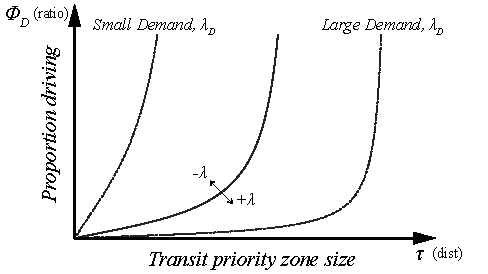
\includegraphics[width=\textwidth]{diagram_tau_pd}
         \caption{Driving proportion function $\Phi_D(\tau)$}
         \label{fig:taupd}
     \end{subfigure}
     \hfill
     \begin{subfigure}[b]{0.45\textwidth}
         \centering
         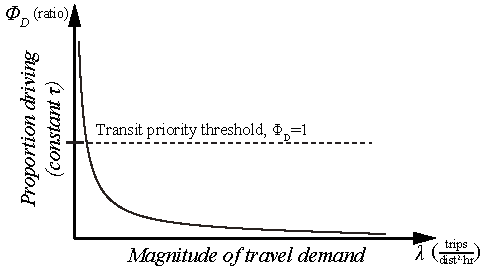
\includegraphics[width=\textwidth]{diagram_demand_pd}
        \caption{Demand magnitude effect when $\tau$ is constant}
         \label{fig:demandpd}
     \end{subfigure}
     \hfill
     \caption{Demand magnitude effect on proportion}
\end{figure}


\section{Numeric application}
To demonstrate the hypothetical outcomes of a pedestrianized zone surrounded by a transit priority zone, numeric input parameters provided in Table~\ref{tab:inputpars} for calculation. These parameters are loosely derived from a real-world case in Melbourne, Australia, shown in Figure~\ref{fig:mel_vicmap}.

\begin{figure}[H]
    \centering
     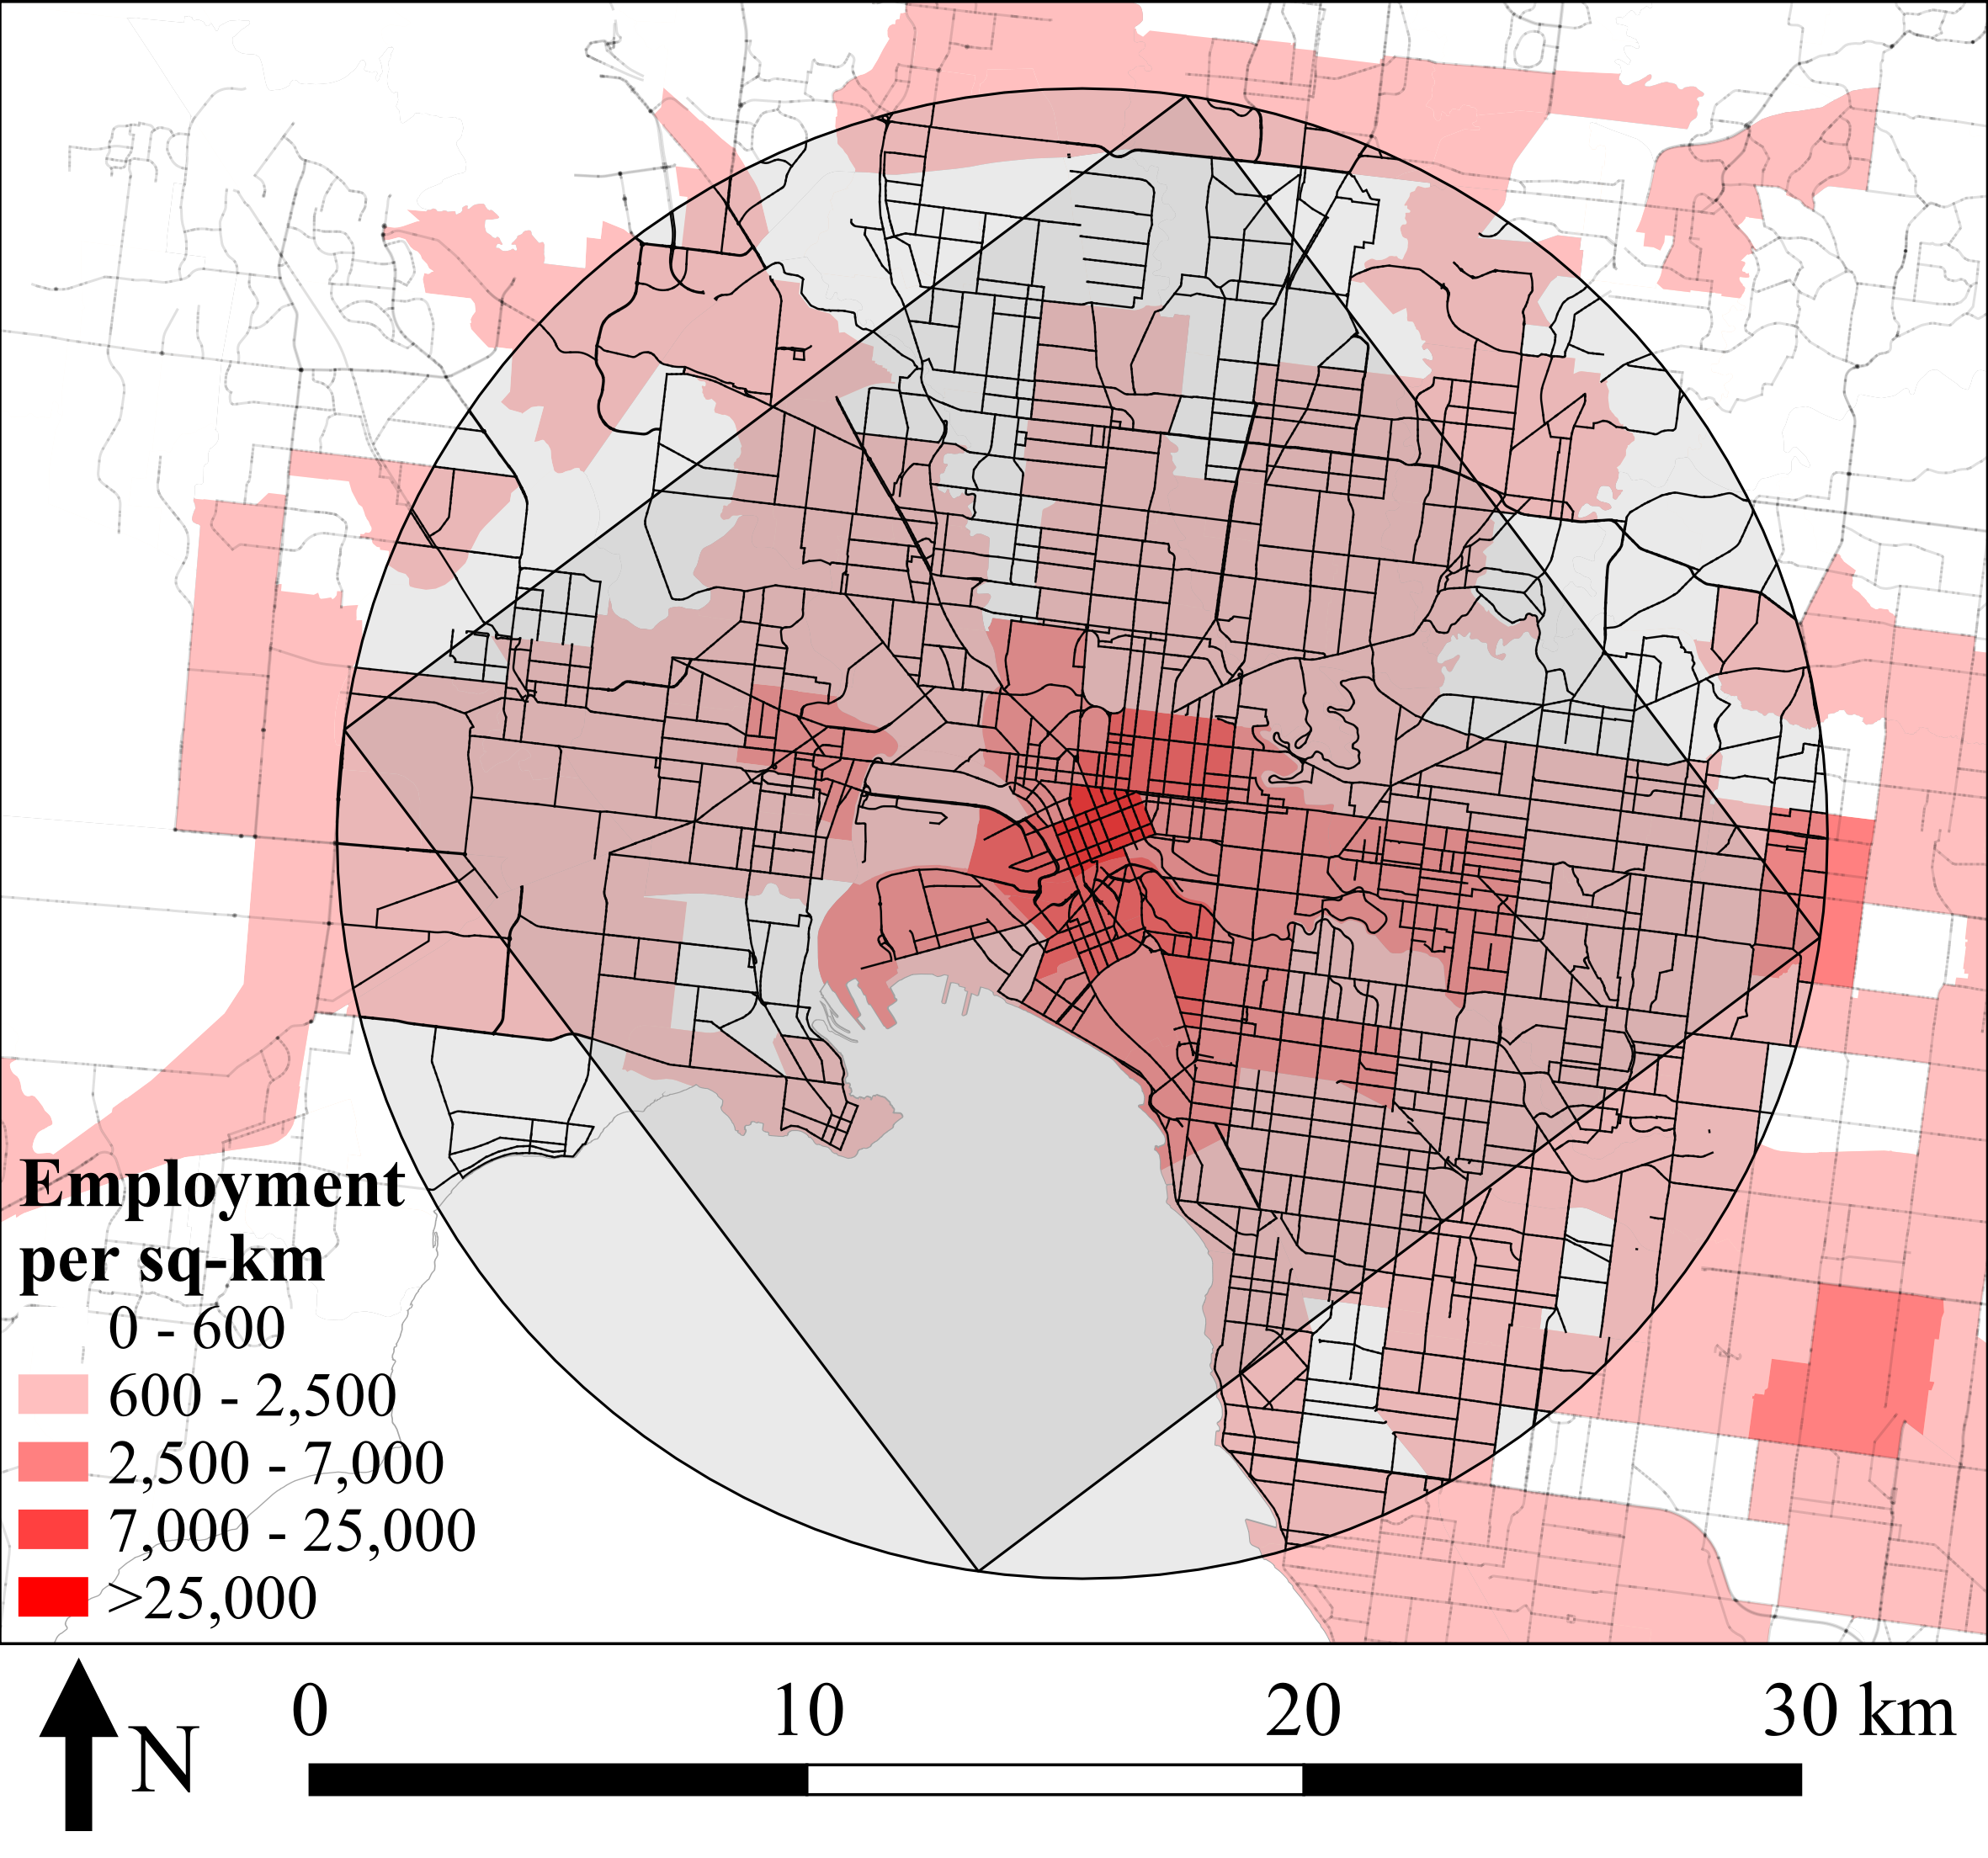
\includegraphics[width=0.5\textwidth]{mel_vicmap}
    \caption{Street Network and Employment Density in Melbourne, Australia}
    \label{fig:mel_vicmap}
\end{figure}

Melbourne provides a useful example to draw from because it is a highly monocentric and automobile dependent city with a sprawling and relatively uniform rectilinear street network with few geographic interruptions other than the bay. This enables parameters to be determined fairly easily using Geospatial Information Systems (GIS) and census sources. Moreover, Melbourne also currently has a partially pedestrianized Central Business District (CBD) and a large mixed-traffic streetcar system (called trams in Australia) which suffers from congestion, making it an intriguing case to draw from.

\begin{table}[H]
\centering\small
\caption{Input Parameters}
\begin{tabular}{ccc}
\toprule
Parameter   & Value & Units \\ \hline
$R$         & 15			& $km$                              \\
$\delta$    & 2.8 		& $\sfrac{lane\cdot dist}{dist^2}$  \\
$\lambda_b$ & 67	& $\sfrac{trips}{km^2\cdot hr}$     \\
$\lambda_c$ & 60	& $\sfrac{trips}{km^2\cdot hr}$     \\
$v_m$       & 50		& $\sfrac{km}{hr}$                  \\
$v_w$       & 5		& $\sfrac{km}{hr}$                  \\
$t_s$       & 60	& $sec$                              \\
$s$         & 0.5			& $km$                              \\
$k_c$       & 45		& $\sfrac{veh}{k}$                  \\
$q_c$       & 500		& $\sfrac{trips}{lane \cdot hr}$    \\
$d$         & $\sfrac{2}{\delta}=0.714$ & $km$                          \\\bottomrule
\end{tabular}
\label{tab:inputpars}
\end{table}



\subsection{Baseline scenario -- no pedestrian or transit priority policies}
First, a baseline scenario in a city with no pedestrianized or transit priority zones using the numeric parameters from Table~\ref{tab:inputpars}, demand is varied in Figure~\ref{fig:baselinett} by shifting the proportion of total demand that drives or uses transit. Again, for demonstration purposes, this assumes infinite transit capacity. The travel time of both mixed-traffic transit and driving dramatically increase as driving demand increases. This is because the network reaches capacity and traffic flow breaks down, it causes average travel time for both driving and mixed-traffic transit to dramatically increase.

\begin{figure}[H]
    \centering
\begin{knitrout}
\definecolor{shadecolor}{rgb}{0.969, 0.969, 0.969}\color{fgcolor}
\includegraphics[width=0.66\textwidth]{figure/baselinett-1} 
\end{knitrout}
    \caption{Average total travel time varying demand with no pedestrian zone or transit priority}
    \label{fig:baselinett}
\end{figure}

It is also clear that transit demand is always slower than driving demand, even if the difference between the two modes becomes arbitrarily small as the average travel time becomes dramatically large. This numerically illustrates the situation hypothesized in Figure~\ref{fig:transittraveltime}. As mentioned, the problem in this scheme is there is little or no incentive for an individual to choose transit, other than out of necessity or to altruistically improve the system for all. 


\subsection{Independent pedestrian and transit priority policies}
While it is unrealistic that travel time would approach infinity, one might assume that as traffic flow breaks down and travel time dramatically increases, demand for travel itself might simply become suppressed in general. To avoid such a scenario, ensuring that travel demand is not suppressed and able to travel freely, the city might decide to impose a pedestrianized or transit priority zone. Figure~\ref{fig:modett} demonstrates the effect of pedestrianized and transit priority zones on the respective average travel time of driving and transit.

\begin{figure}[H]
     \centering
     \begin{subfigure}[b]{0.49\textwidth}
         \centering
\begin{knitrout}
\definecolor{shadecolor}{rgb}{0.969, 0.969, 0.969}\color{fgcolor}
\includegraphics[width=\maxwidth]{figure/drivett-1} 
\end{knitrout}
         \caption{Effect of pedestrian zone size on average driving travel time (no transit priority zone)}
         \label{fig:ttpedzone}
     \end{subfigure}
     \hfill
     \begin{subfigure}[b]{0.49\textwidth}
         \centering
\begin{knitrout}
\definecolor{shadecolor}{rgb}{0.969, 0.969, 0.969}\color{fgcolor}
\includegraphics[width=\maxwidth]{figure/transittt-1} 
\end{knitrout}
        \caption{Effect of transit priority zone size on average transit travel time (no pedestrian zone)}
         \label{fig:tttransitzone}
     \end{subfigure}
        \caption{Average travel time by mode varying pedestrian and transit zone size, $\gamma$ and $\tau$}
        \label{fig:modett}
\end{figure}

Both Figures~\ref{fig:ttpedzone} and~\ref{fig:tttransitzone} decrease in travel time as the zone sizes increase. This is because the most extreme congestion in the very center of the city is effectively abolished, thus yielding a huge improvement but with diminishing returns. However, in the driving case the travel time begins to increase as the pedestrianized zone become unreasonably large, effectively trading driving for walking. 

A caveat in this model is that both Figures~\ref{fig:ttpedzone} and~\ref{fig:tttransitzone} approach infinity as the zone size becomes infinitesimally small. From a mathematical perspective, this is an artifact of the piece-wise monotonic function approaching infinity as the travel demand exceeds available roadway capacity on the perimeter road (i.e., when $q \geq q_c:~t(q)=t_c \left(\sfrac{q}{q_c}\right)^{20}$). More intuitively, this extreme boundary condition occurs when the pedestrian or transit priority zone becomes so small that there simply is not enough road infrastructure to carry the vehicles around the city center. 

The reason why Figure~\ref{fig:modett} is unaffected by this condition is that when the pedestrian and transit priority zones are a size of exactly zero, they do not exist at all and do not create this condition. In reality, this is somewhat confounding that traffic congestion would suddenly jump to infinity as a transit or pedestrian zone size increases from zero to some tiny zone size, $\sfrac{d}{d\tau}$. However, one realistic constraint is that a pedestrian or transit priority zone size cannot feasibly be smaller than one city block, or else there would be no road infrastructure to carry the vehicles. Assuming a street spacing of $s$, this can be used to arbitrarily define a boundary for the minimum feasible zone size, $\gamma \geq s$ and $\tau \geq s$, for pedestrian and transit priority zones, respectively. 


\subsection{Transit priority threshold}
To determine whether traffic conditions are worse enough to justify transit priority, regardless of a pedestrianized zone, the driving demand proportion, $\Phi_D$, can be evaluated against the transit priority threshold, $\Phi_D = 1$. To demonstrate the transit priority threshold, Figure~\ref{fig:demandload} shows a range of transit priority zone sizes across a varying demand load.

\begin{figure}[H]
    \centering
\begin{knitrout}
\definecolor{shadecolor}{rgb}{0.969, 0.969, 0.969}\color{fgcolor}
\includegraphics[width=0.66\textwidth]{figure/demandload-1} 
\end{knitrout}
    \caption{Demand loading to justify transit priority}
    \label{fig:demandload}
\end{figure}

Figure~\ref{fig:demandload} shows that as demand load increases, the threshold decreases (as also shown in Figure~\ref{fig:demandpd}). Conversely, as the transit priority zone becomes larger (e.g., $\frac{\tau}{R}$ from 0.05 to 0.20), the threshold effectively increases. This is because traffic congestion decreases further from the center. However, this also means that just because a large transit priority zone of a certain size does not meet the threshold, it does not mean transit priority is entirely inappropriate, only that a smaller zone may be required. 


\subsection{Combined pedestrian and transit priority policies}
Figures~\ref{fig:ttpedzone} and~\ref{fig:tttransitzone} only consider travel time independently of the modes, and does not consider the combined effect on the average travel time of both modes. Meaning, they do not account for the effect that a pedestrian zone might have on travel time with a transit zone and vice versa. Figure~\ref{fig:combott} shows the combined average travel for both modes as the pedestrianized and transit priority zone vary in size. For demonstration, the transit priority zone is shown as being some proportion of the pedestrian zone, ranging from being the same size as the pedestrian zone (i.e., no transit priority zone) to four times the size of the pedestrianized zone.

\begin{figure}[H]
\centering
\begin{knitrout}
\definecolor{shadecolor}{rgb}{0.969, 0.969, 0.969}\color{fgcolor}
\includegraphics[width=0.66\textwidth]{figure/combott-1} 
\end{knitrout}
    \caption{Average combined travel time for transit and driving varying $\tau$ and $\gamma$}
    \label{fig:combott}
\end{figure}

\subsection{Optimal pedestrian and transit priority zone sizes}
It is clear from Figure~\ref{fig:combott} that the optimal travel time can vary with both the pedestrianized and transit priority zone sizes. To visualize this bi-variate gradient, the travel time in Figure~\ref{fig:optimal} is plotted against both the pedestrian zone on the horizontal axis, and the transit priority zone on the vertical axis. The shaded diagonal half of the plot represents when the transit priority zone is less than the pedestrian zone size. While a result can be calculated, it makes little sense in reality to have such a condition. Thus, any point below the diagonal can be considered outside of feasible space, simplifying optimization.

\begin{figure}[H]
    \centering
\begin{knitrout}
\definecolor{shadecolor}{rgb}{0.969, 0.969, 0.969}\color{fgcolor}
\includegraphics[width=\textwidth]{figure/optimalpars-1} 
\end{knitrout}
    \caption{Average total travel time varying across $\gamma$ and $\tau$}
    \label{fig:optimal}
\end{figure}

In this case, the optimal pedestrianized and transit priority zone sizes are 16\% and 43\% of $R$, respectively; with a minimum average travel time of 0.92 hours. It is interesting that the transit priority zone is only 170\% larger (27\% of R) than the pedestrianized zone. This suggests that the majority of the travel time improvement is achieved through pedestrianization, and that the transit priority zone mainly serves to mitigate the perimeter road congestion. The optimal travel time gradient surface in Figure~\ref{fig:optimal} is also fairly stable, allowing room for error. Slightly over sized zones would not result in any appreciable loss in performance.


\subsection{Network capacity of combined pedestrian and transit priority policies}
Recalling the breakdown of traffic flow in Figure~\ref{fig:baselinett}, the optimal policy for a varying demand loading is shown in comparison in Figure~\ref{fig:comparett}. The optimal case not only provides a lower average travel time initially, but also does not break down as severely. After a certain level of demand the optimal travel time appears to plateau, this is because the entire city has been zoned as transit priority, establishing a stable travel average time. If the total city extents were larger (i.e., a larger $R$), the optimal case might continue its gradual increase. However, a larger city extent would mean the traffic density in the city center is proportionally increased, thus worsening the breakdown point. 

\begin{figure}[H]
    \centering
\begin{knitrout}
\definecolor{shadecolor}{rgb}{0.969, 0.969, 0.969}\color{fgcolor}
\includegraphics[width=0.66\textwidth]{figure/comparett-1} 
\end{knitrout}
    \caption{Comparing average total travel time for no policy and optimal pedestrian and transit priority policies}
    \label{fig:comparett}
\end{figure}


\subsection{Supplemental comparative analysis}
To further explore the relative application of the proposed model beyond Melbourne, Australia; six additional cities are analyzed. These six cities are Tucson, Arizona; Sacramento, California; Fresno, California; Las Vegas, Nevada; Denver, Colorado; and Chicago, Illinois. As shown in Figure~\ref{fig:vicmap}), all of the cities possess a robust rectilinear street network and some level of monocentricity in the form of centrally concentrated employment density. It is important to note that these densities are employment densities, not housing density. Employment density was chosen to better reflect the relative distribution of trip destinations, regardless of origin.

\pagebreak
\begin{figure}[H]
     \centering
     \begin{subfigure}[b]{0.49\textwidth}
         \centering
		 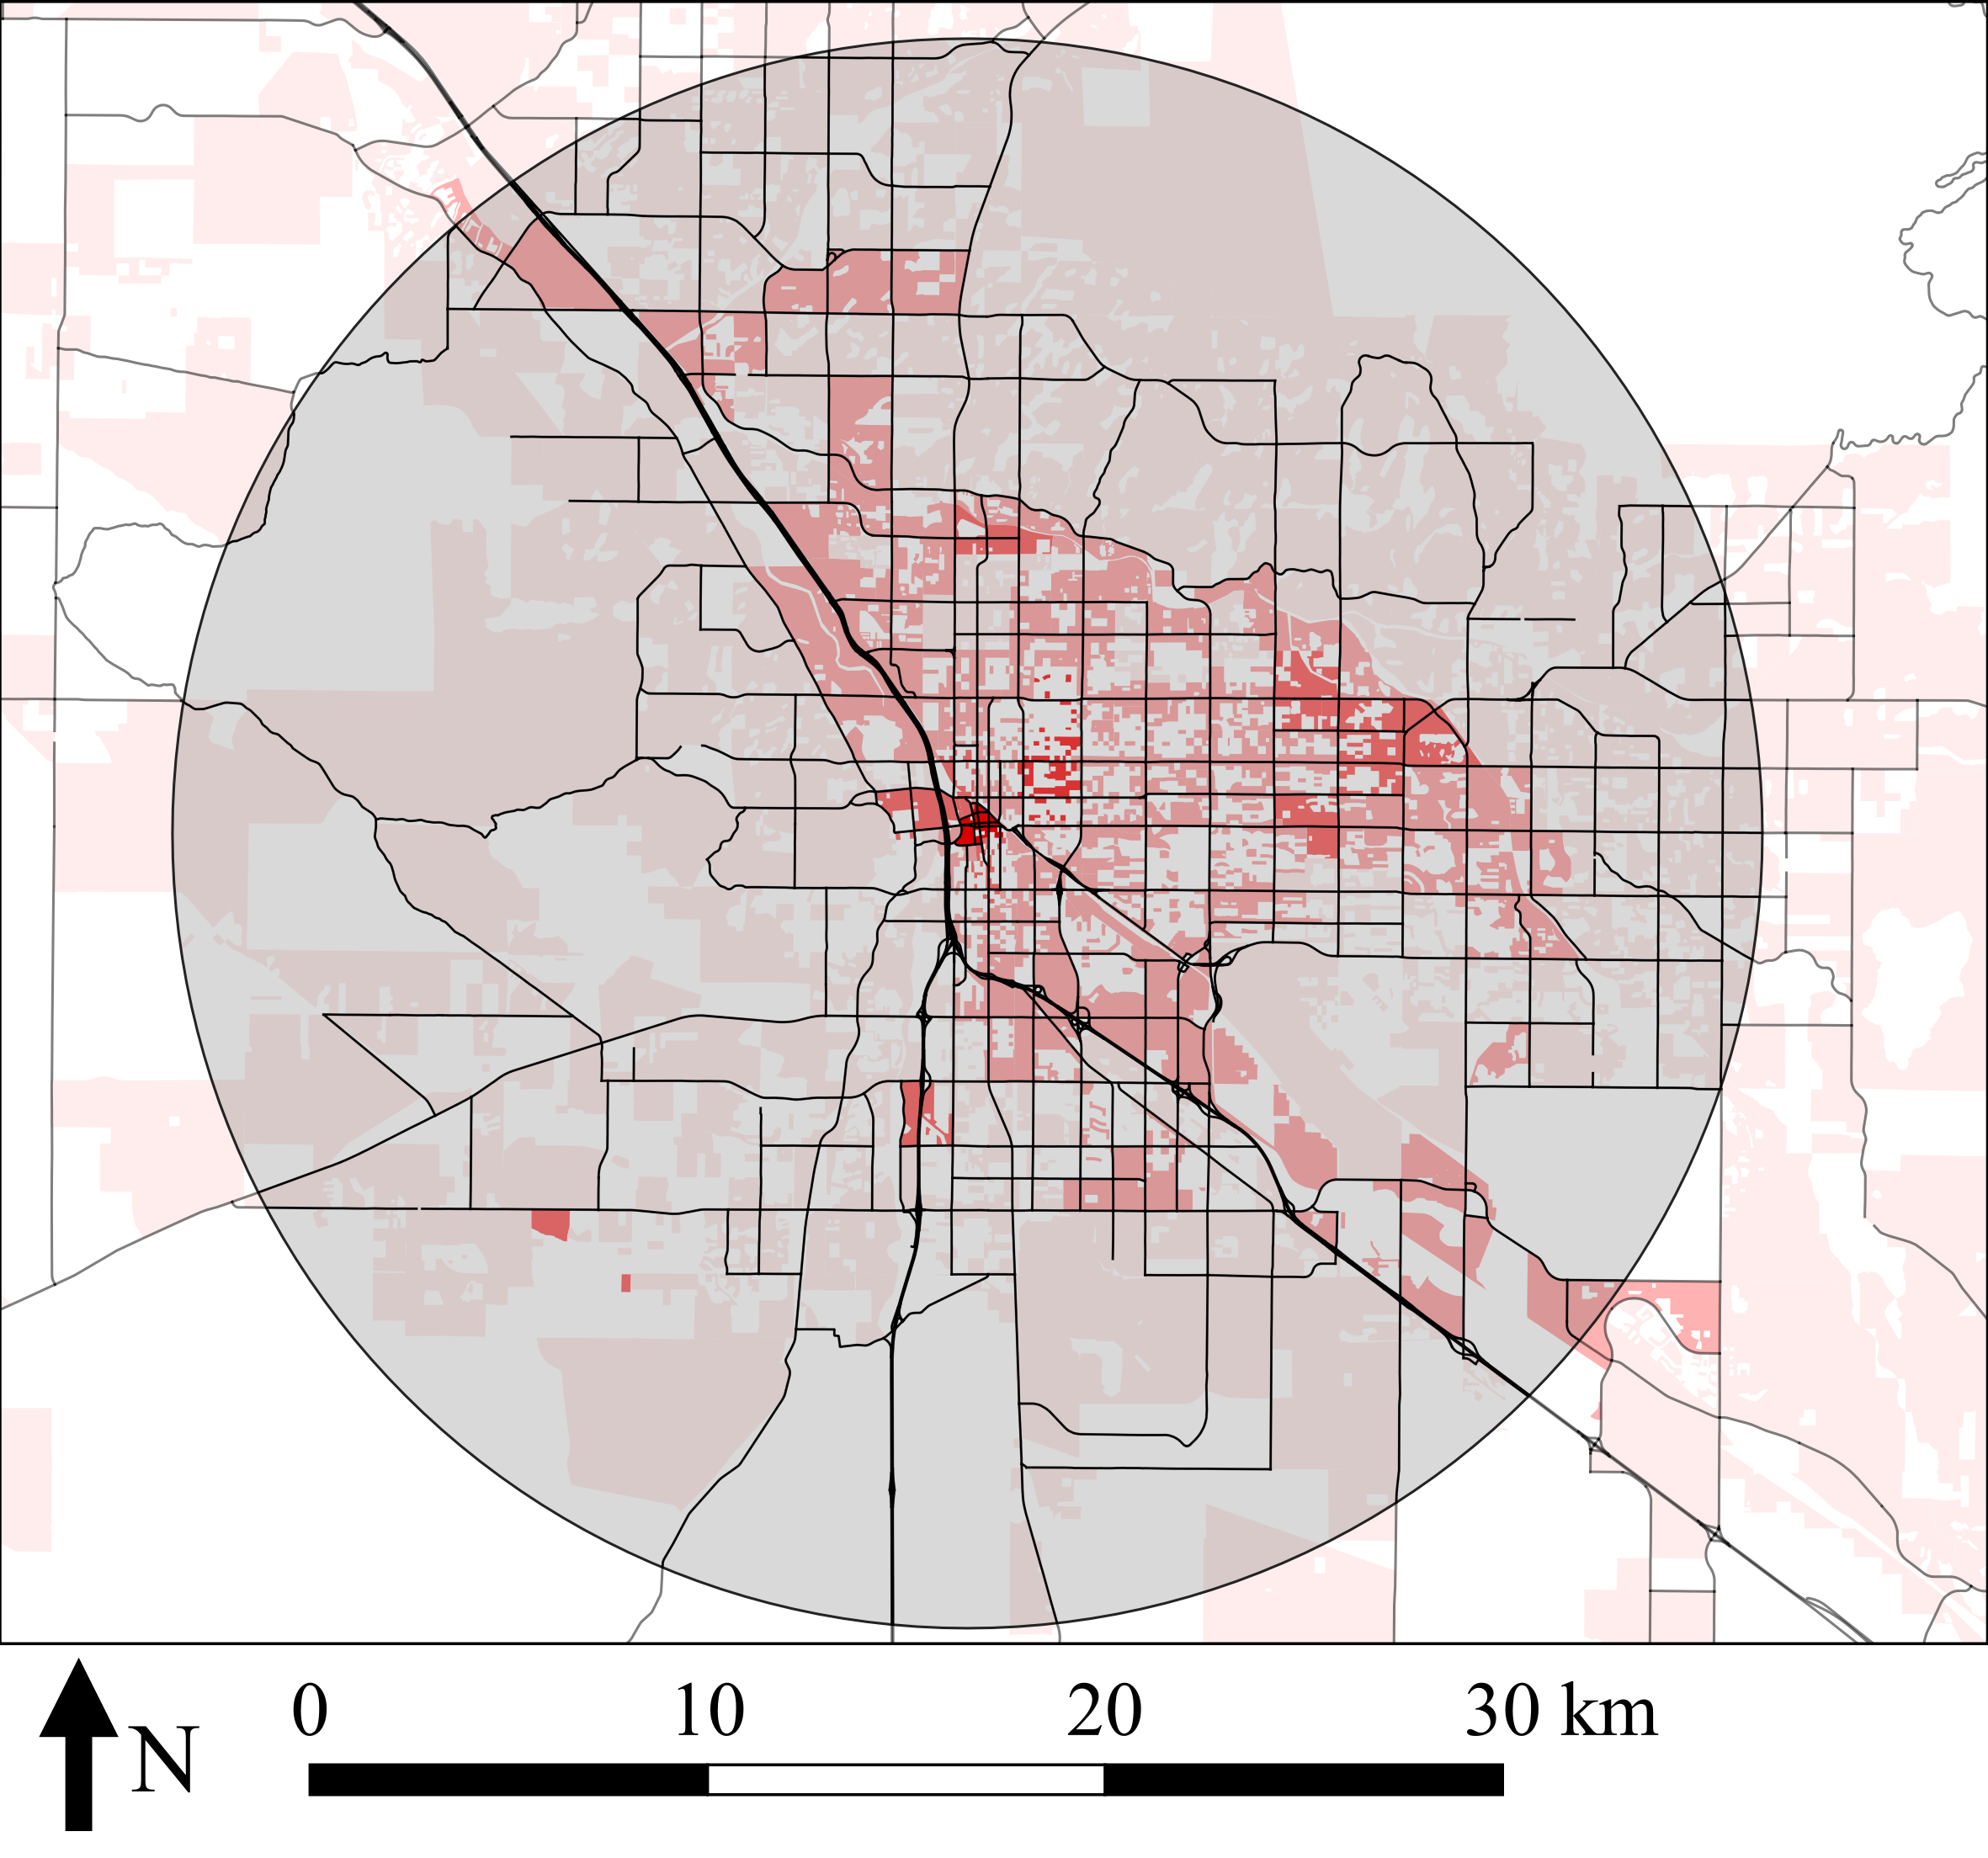
\includegraphics[width=\textwidth]{tuc_vicmap}
        \caption{Tucson, AZ}
         \label{fig:tucmap}
     \end{subfigure}
          \hfill             
     \begin{subfigure}[b]{0.49\textwidth}
         \centering
		 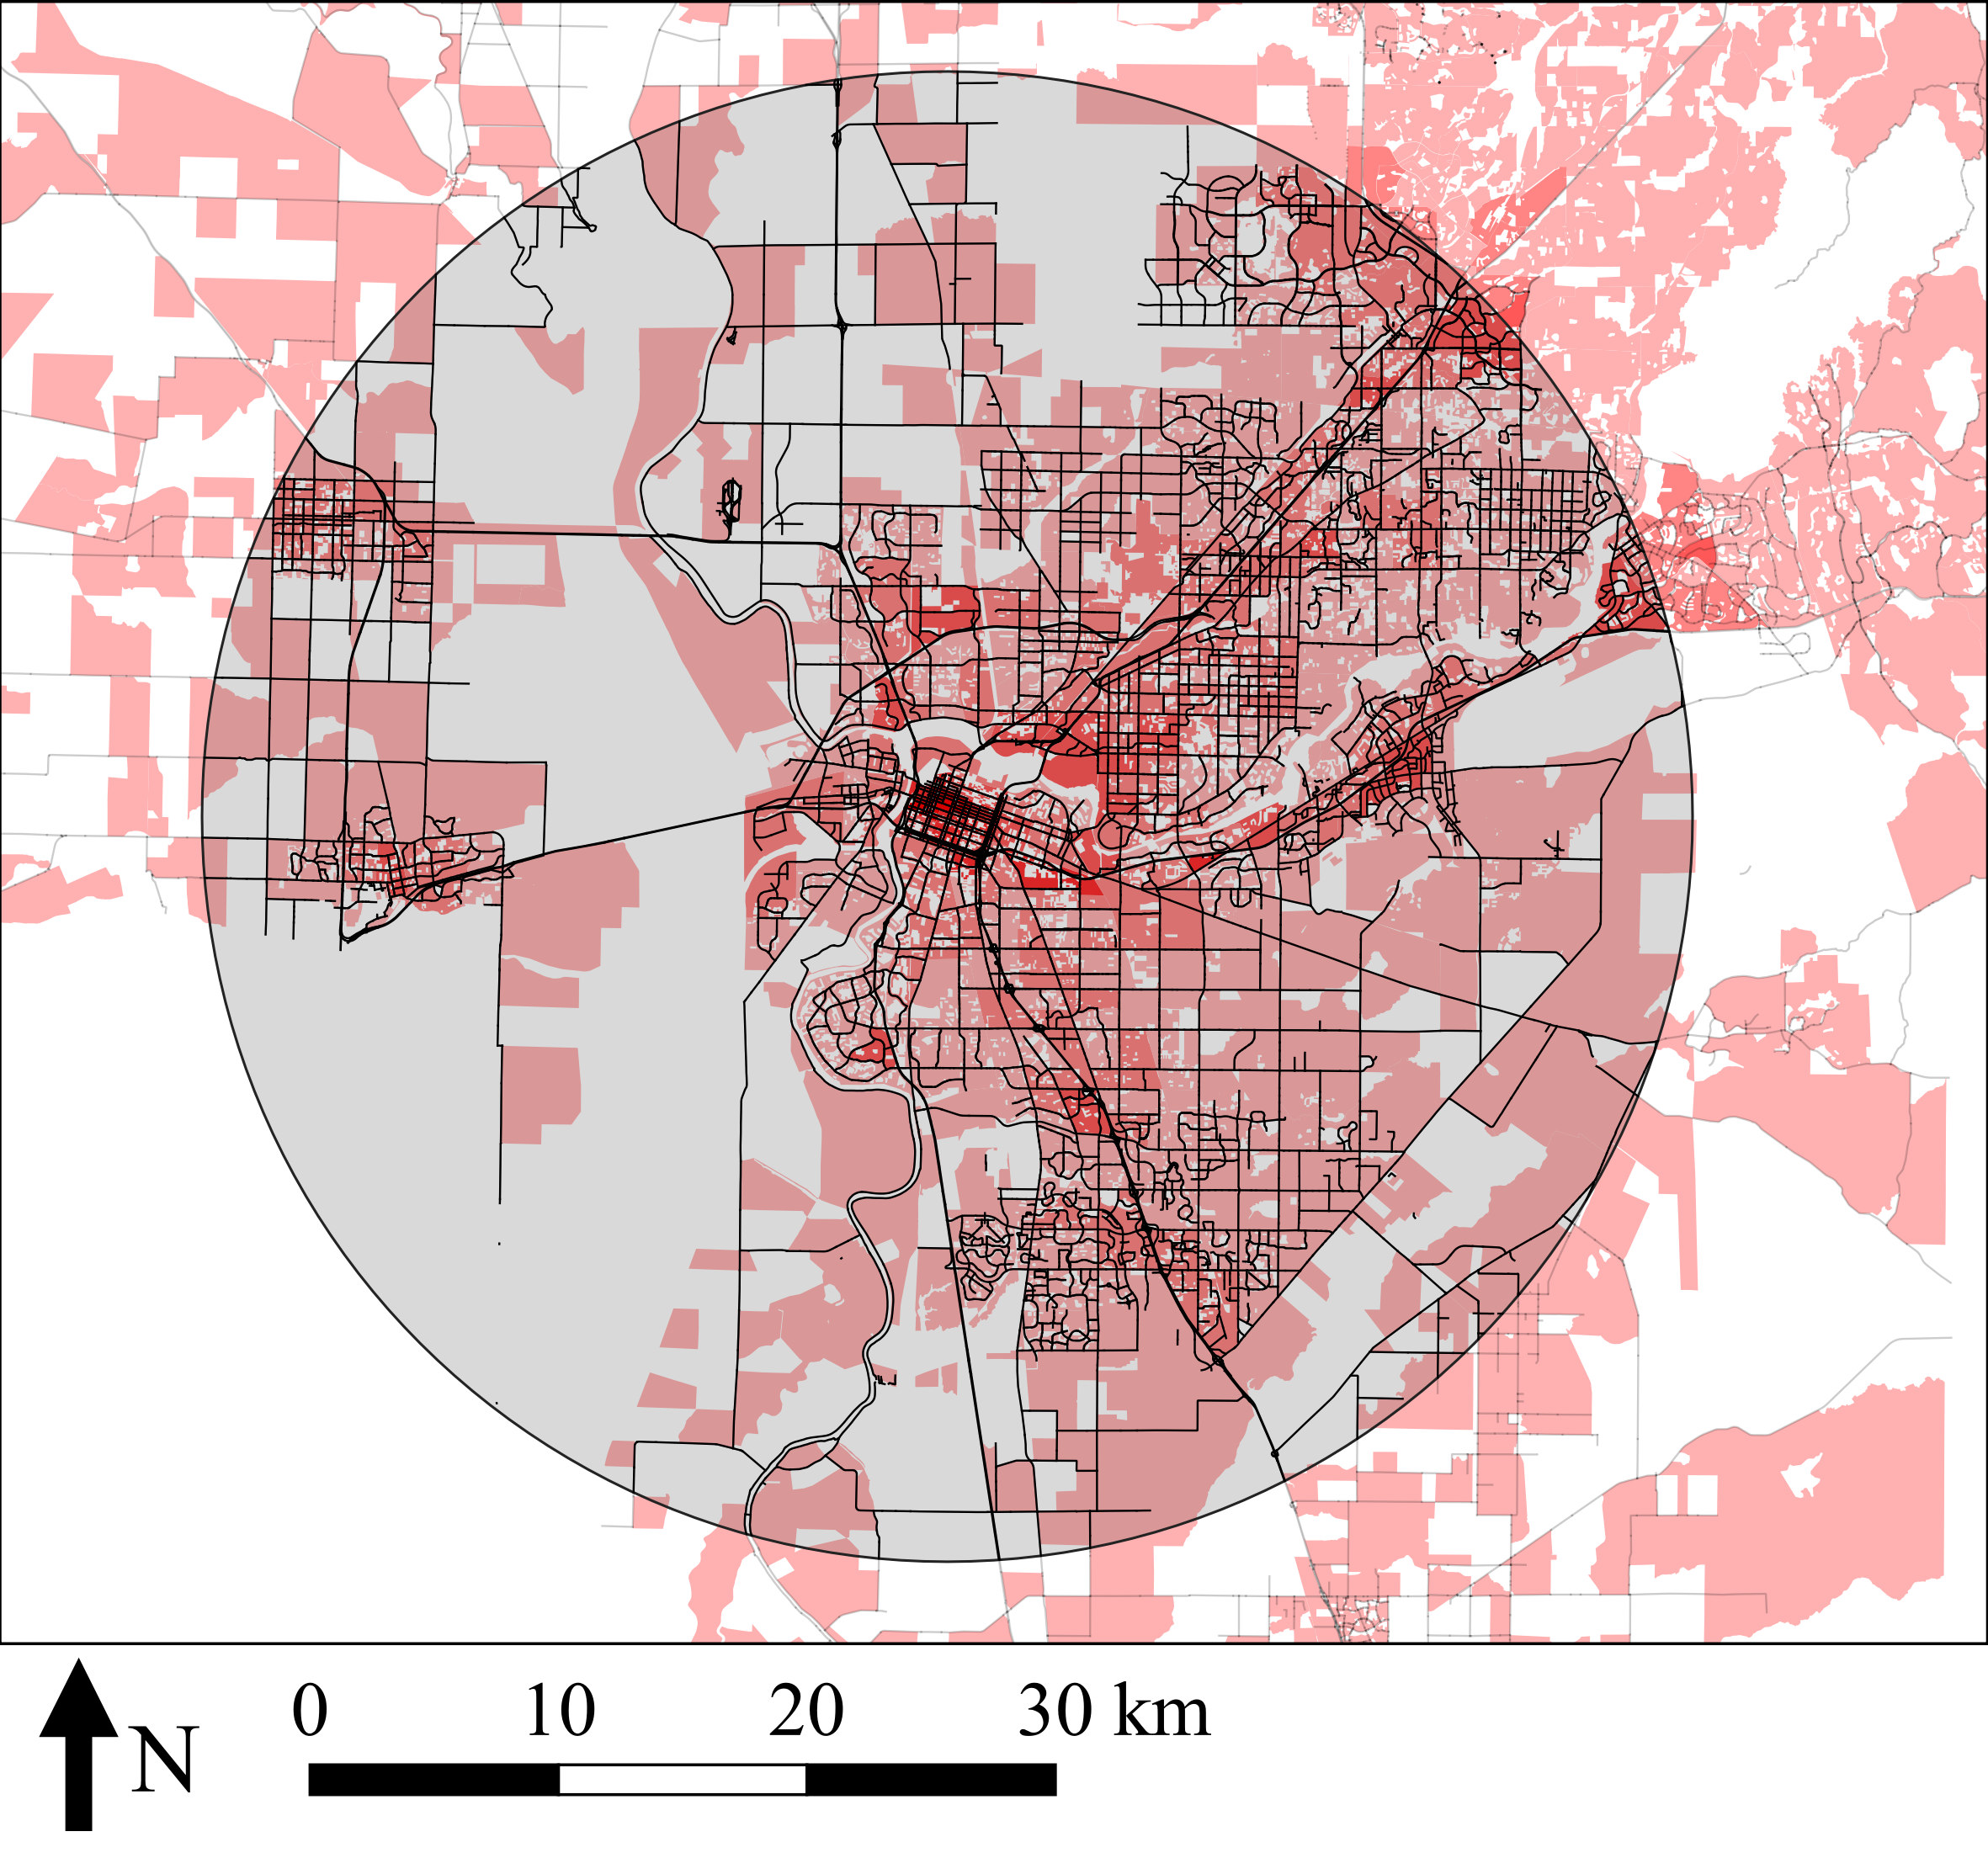
\includegraphics[width=\textwidth]{sac_vicmap}
        \caption{Sacramento, CA}
         \label{fig:sacmap}
     \end{subfigure}
       
     \begin{subfigure}[b]{0.49\textwidth}
         \centering
		 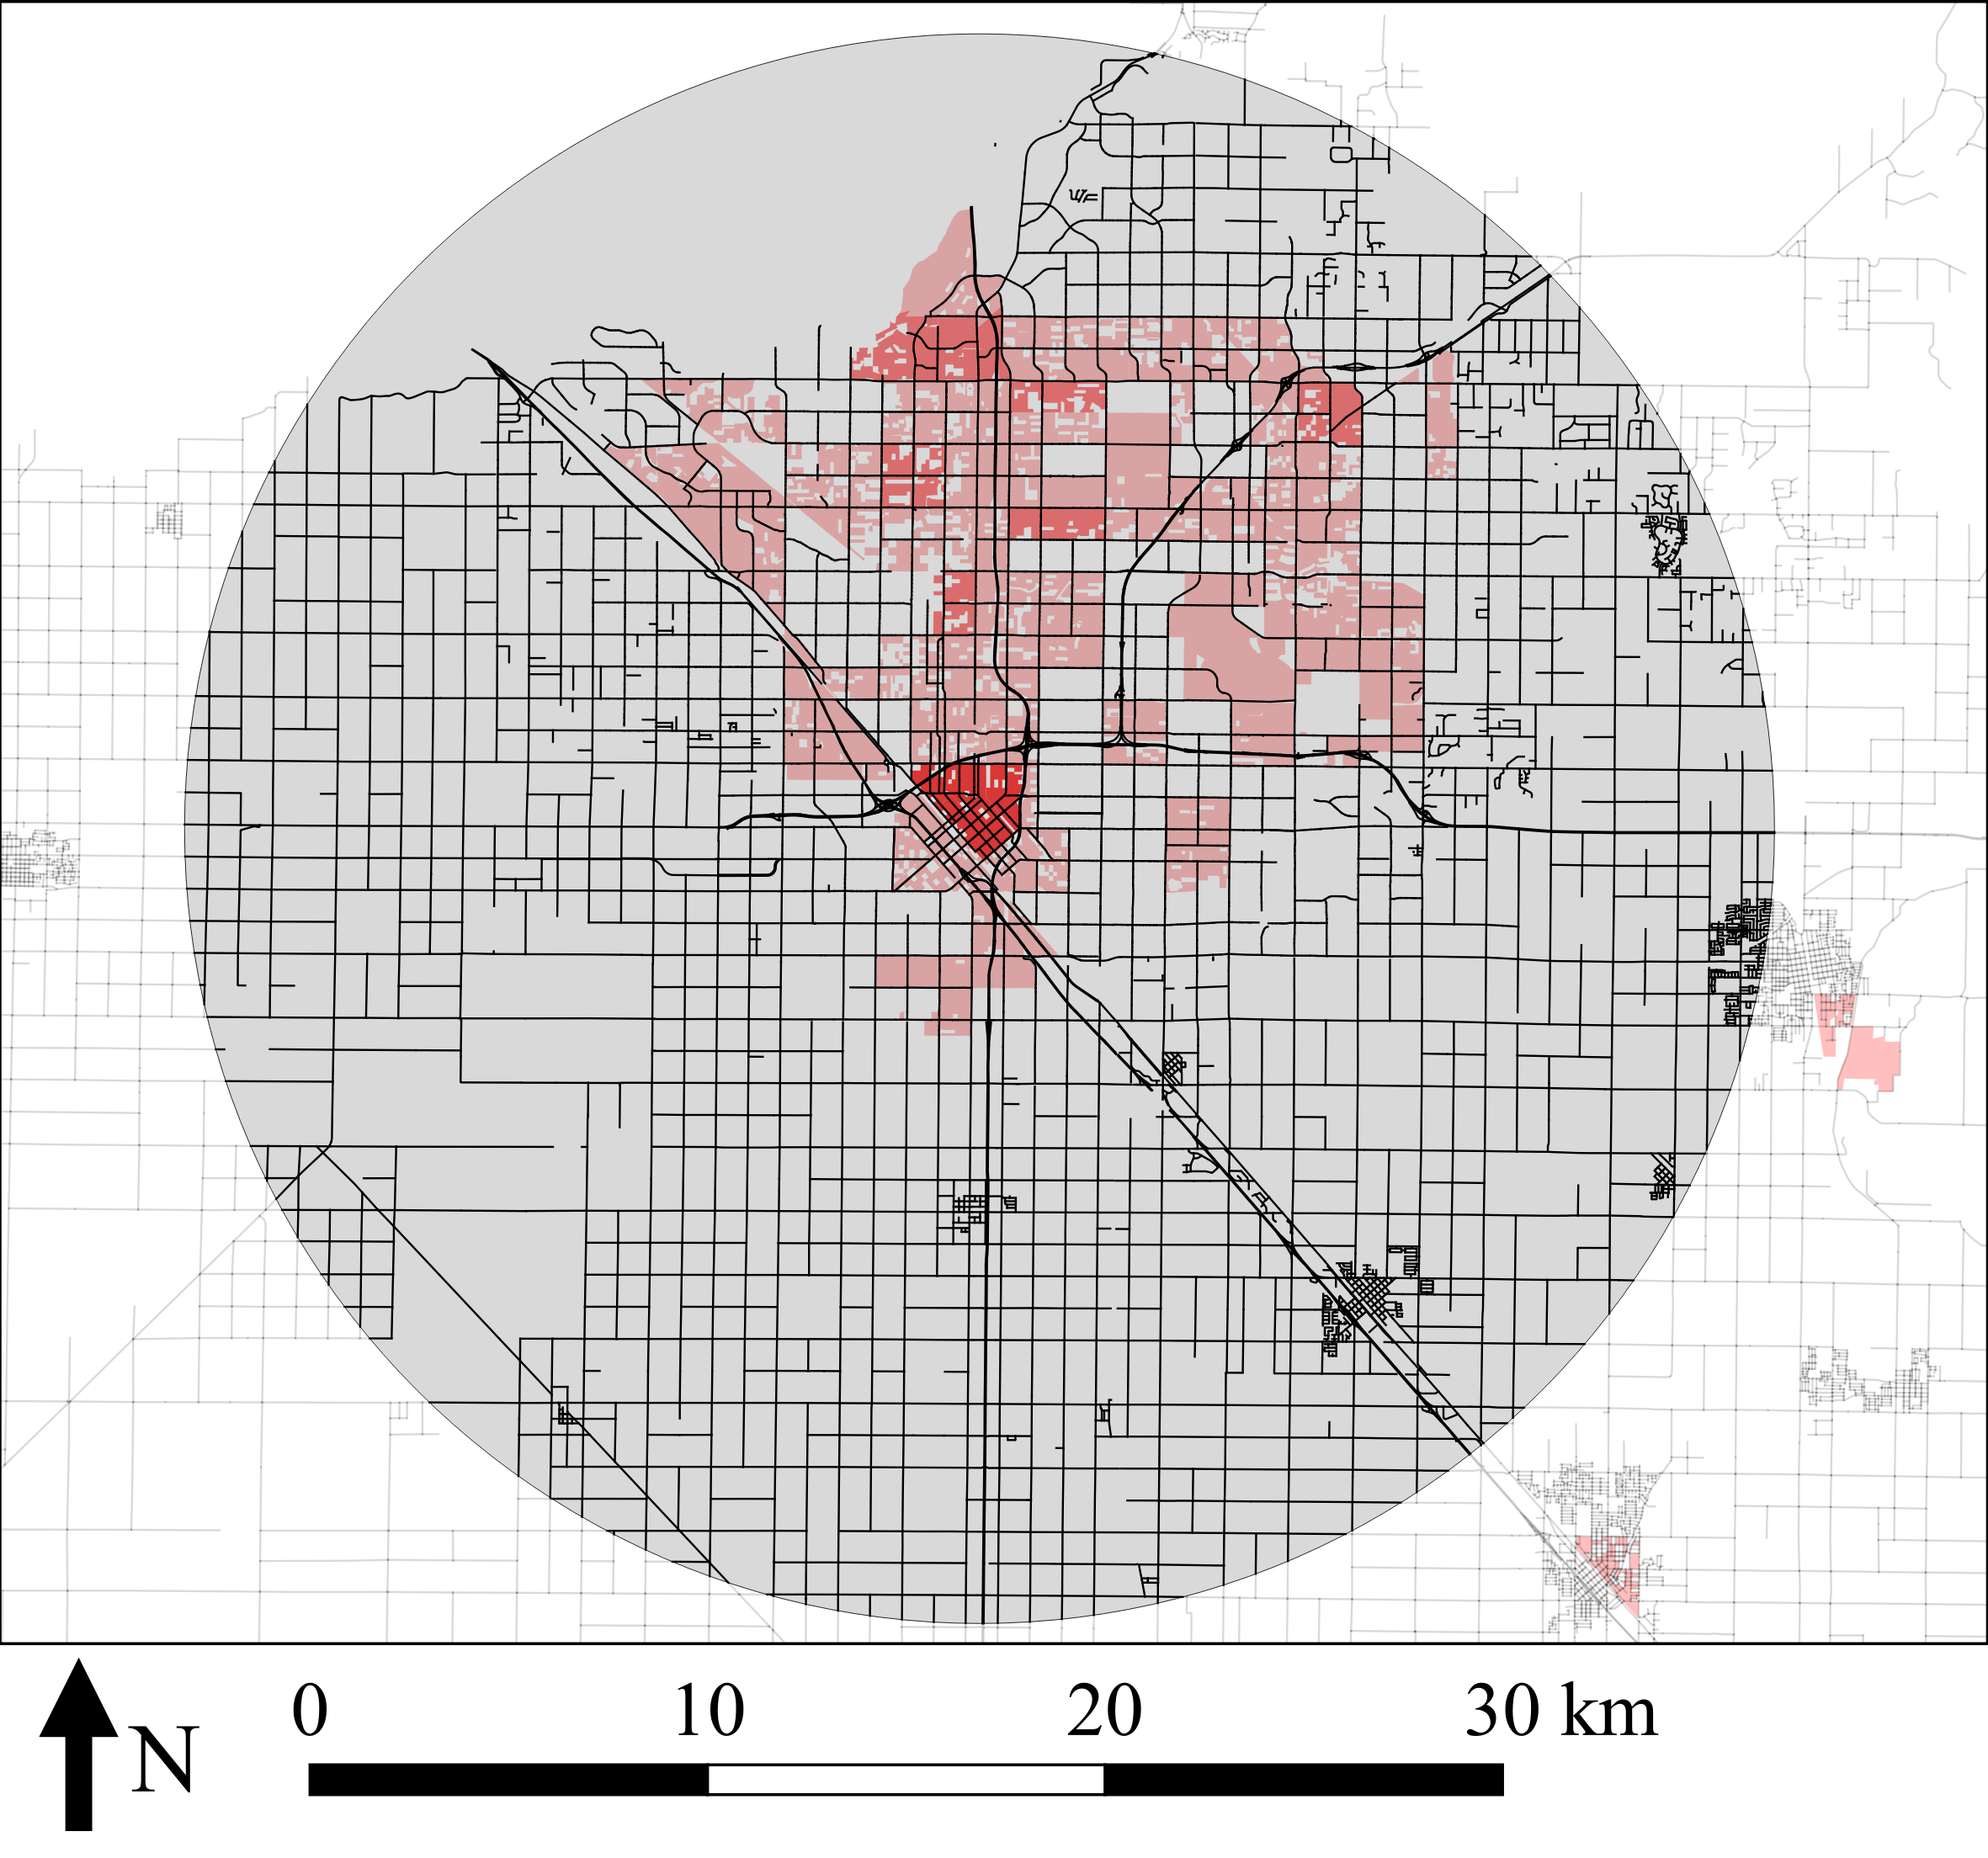
\includegraphics[width=\textwidth]{frs_vicmap}
        \caption{Fresno, CA}
         \label{fig:frsmap}
     \end{subfigure}
          \hfill            
     \begin{subfigure}[b]{0.49\textwidth}
         \centering
		 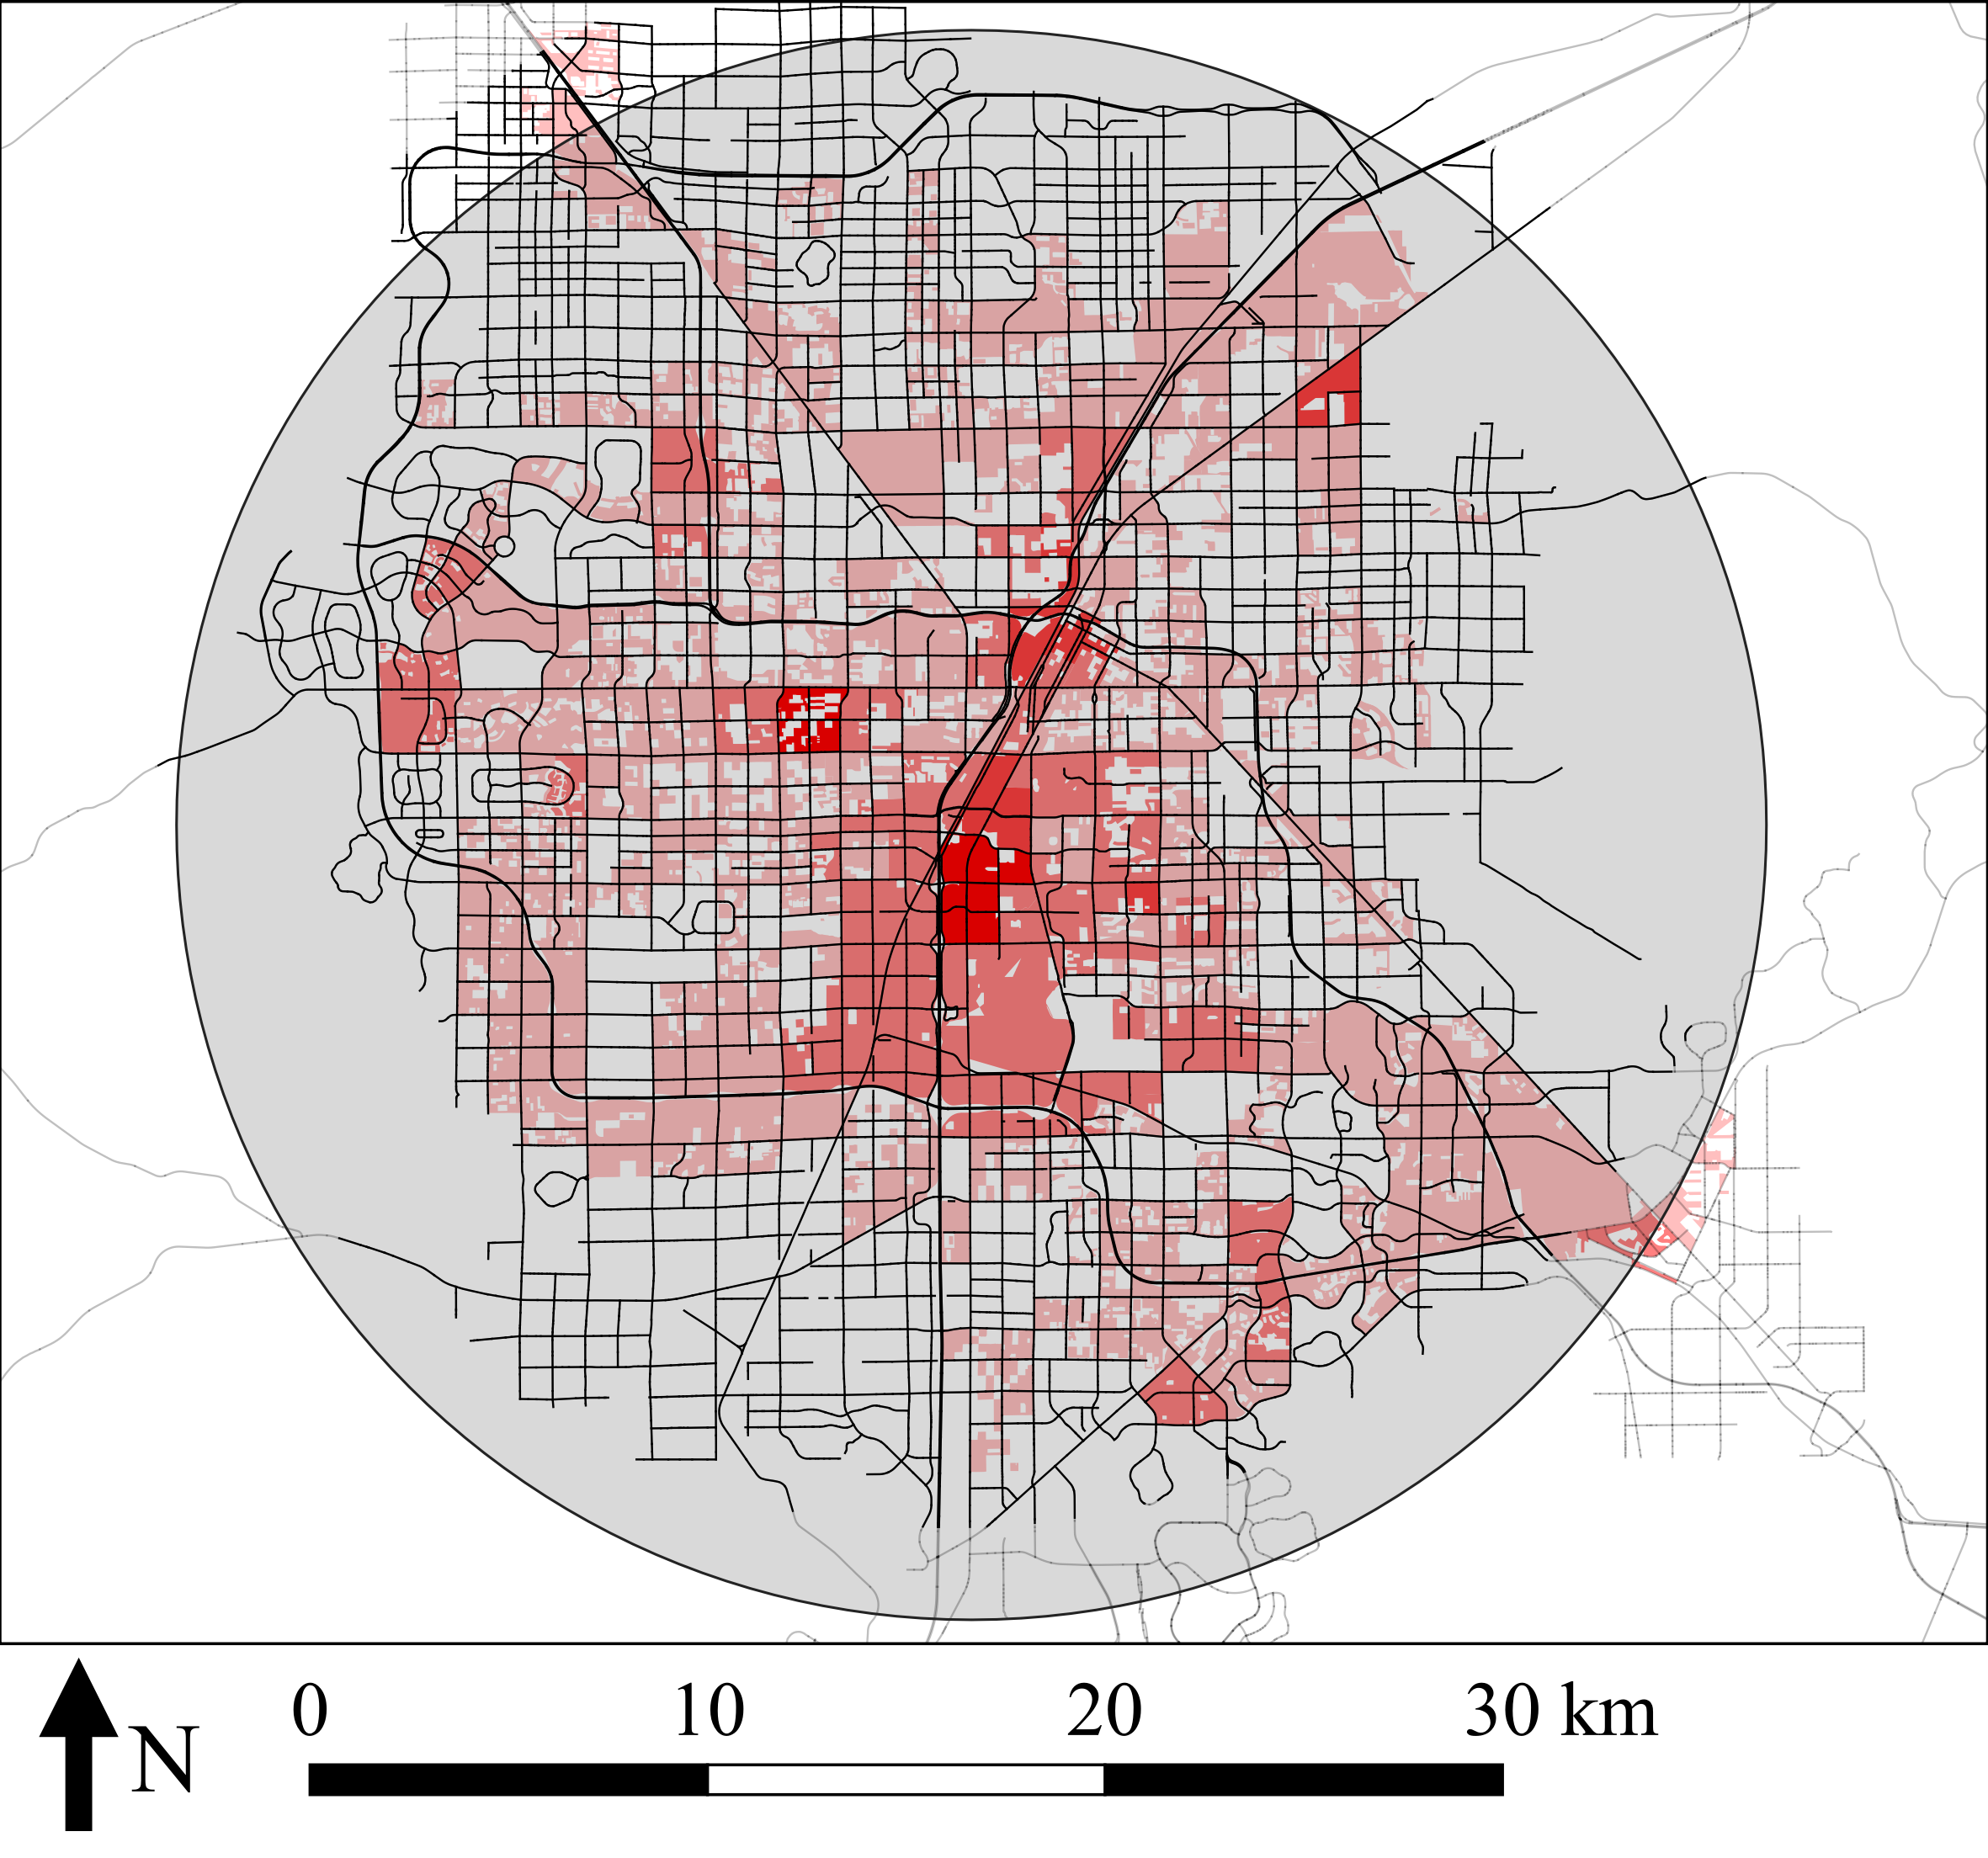
\includegraphics[width=\textwidth]{veg_vicmap}
        \caption{Las Vegas, NV}
         \label{fig:vegmap}
     \end{subfigure}
   
     \begin{subfigure}[b]{0.49\textwidth}
         \centering
		 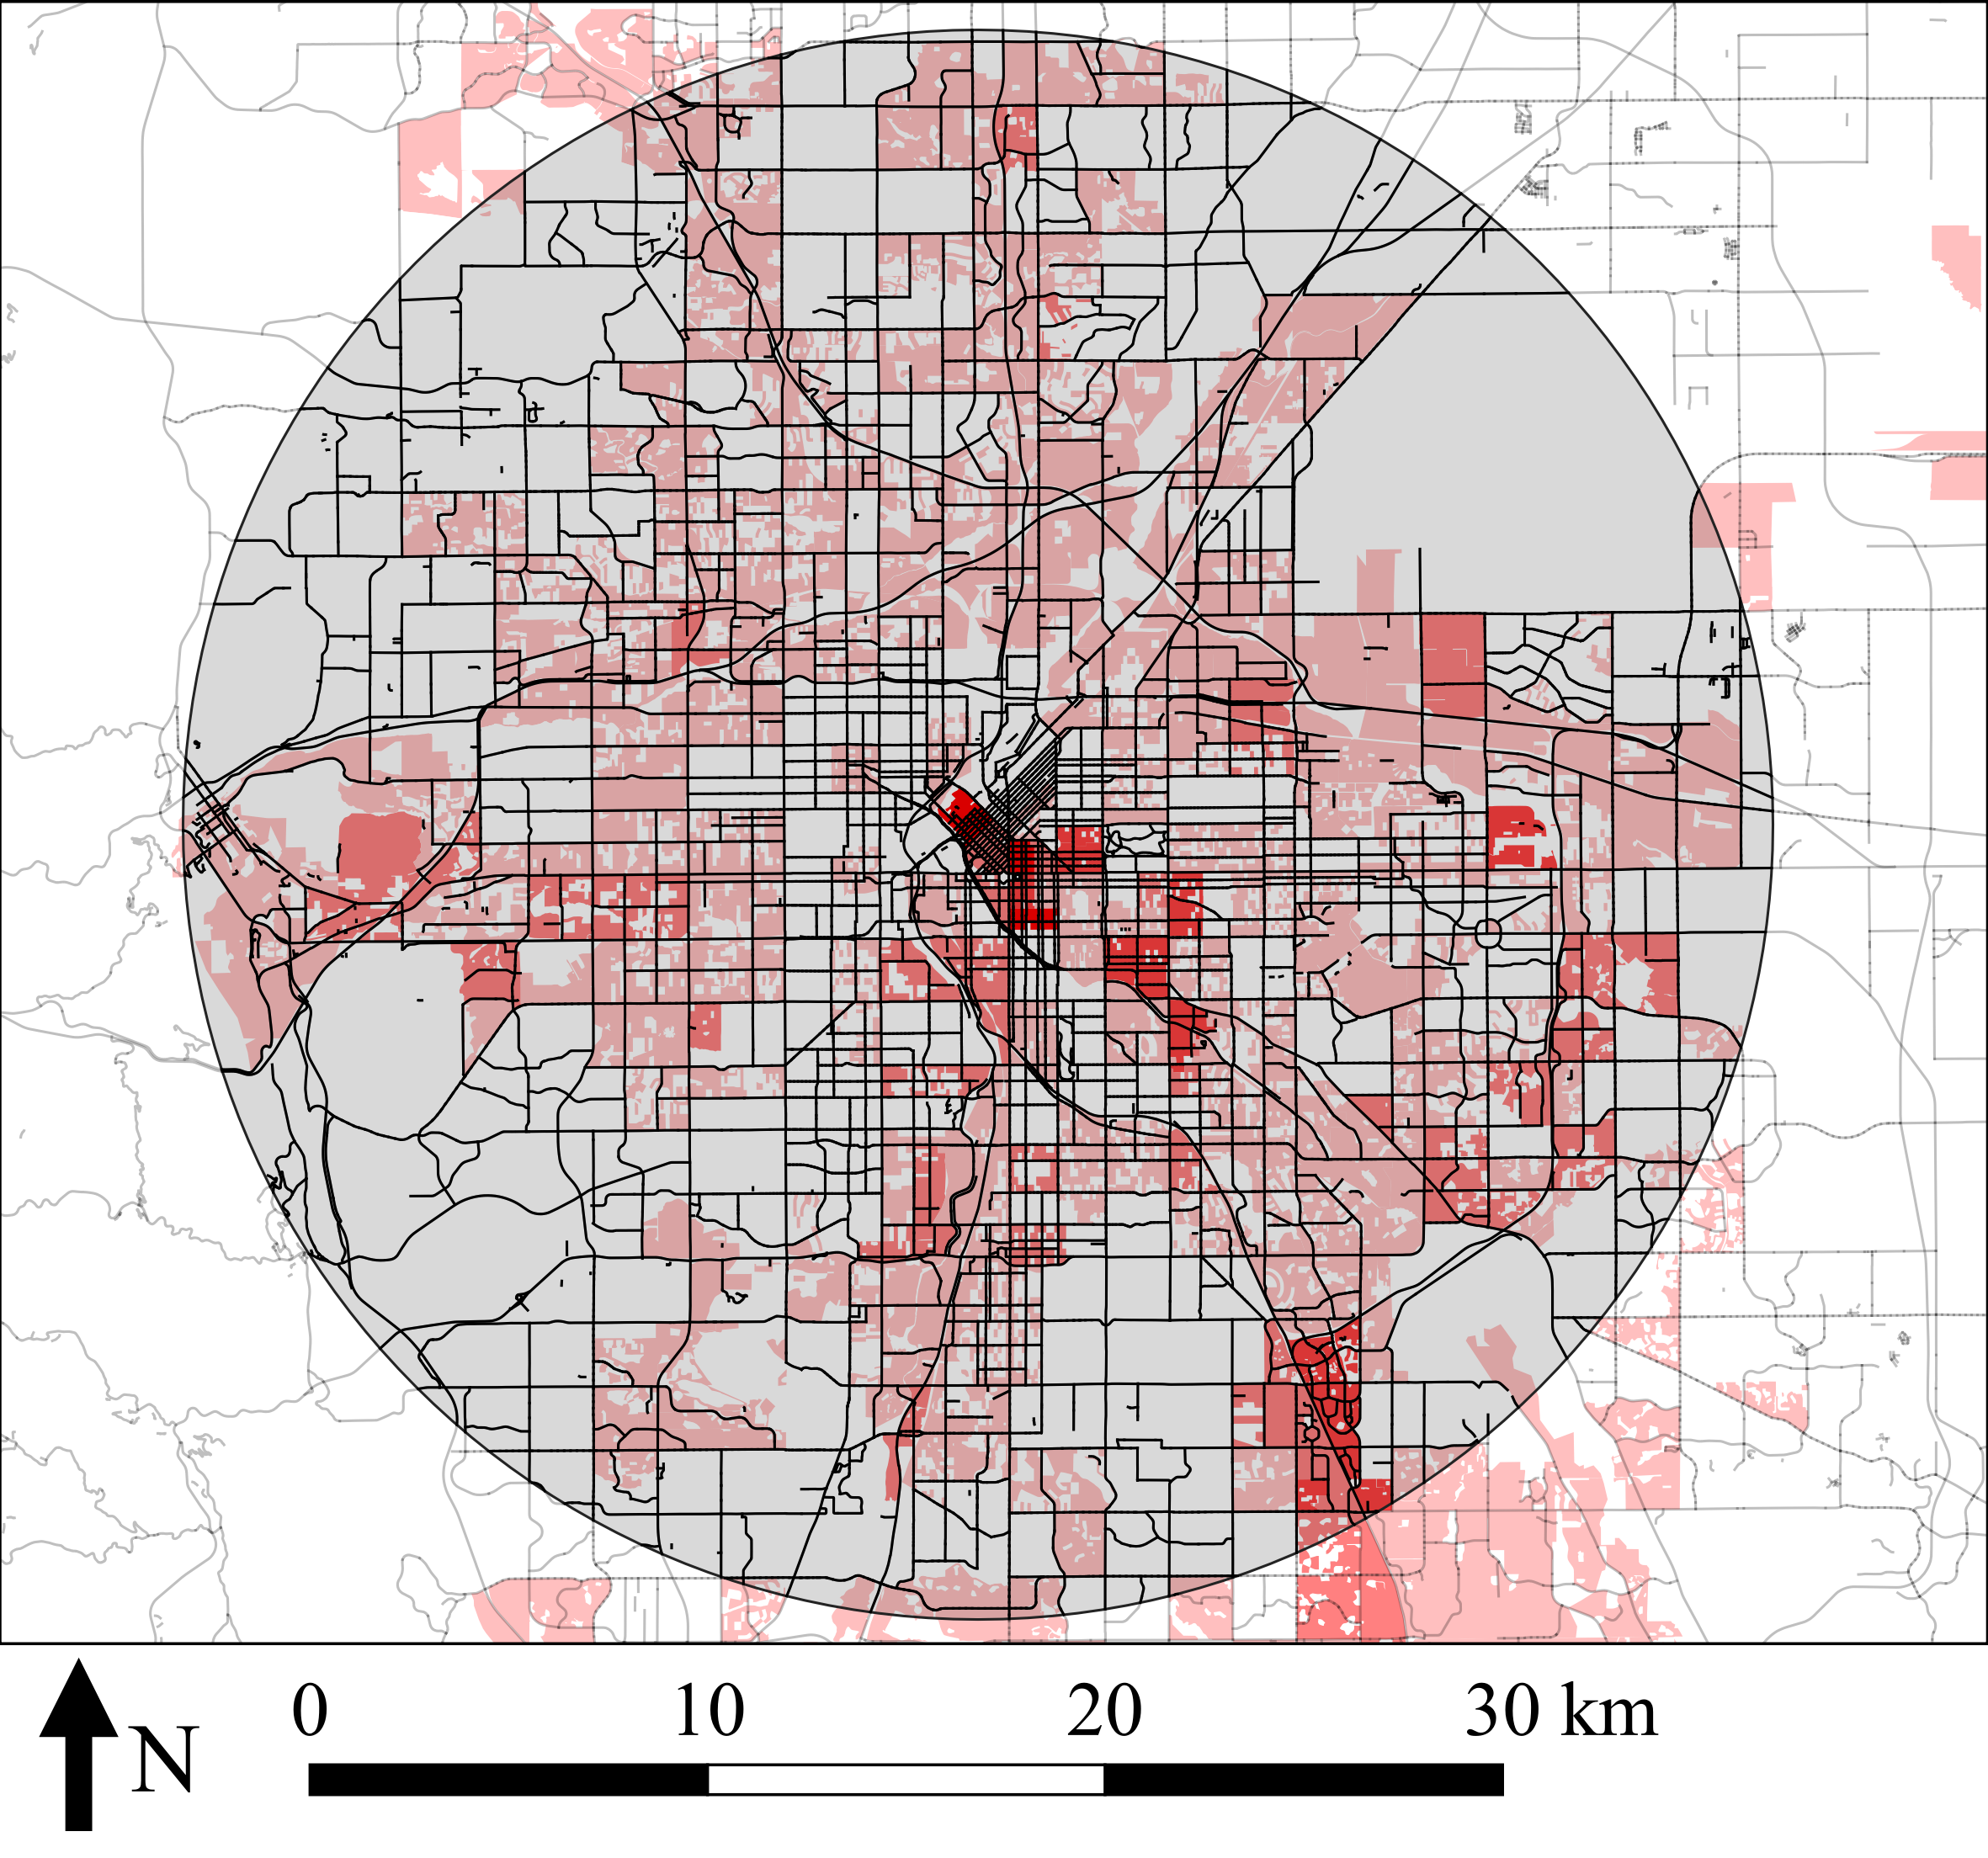
\includegraphics[width=\textwidth]{den_vicmap}
        \caption{Denver, CO}
         \label{fig:denmap}
     \end{subfigure}
         \hfill       
     \begin{subfigure}[b]{0.49\textwidth}
         \centering
		 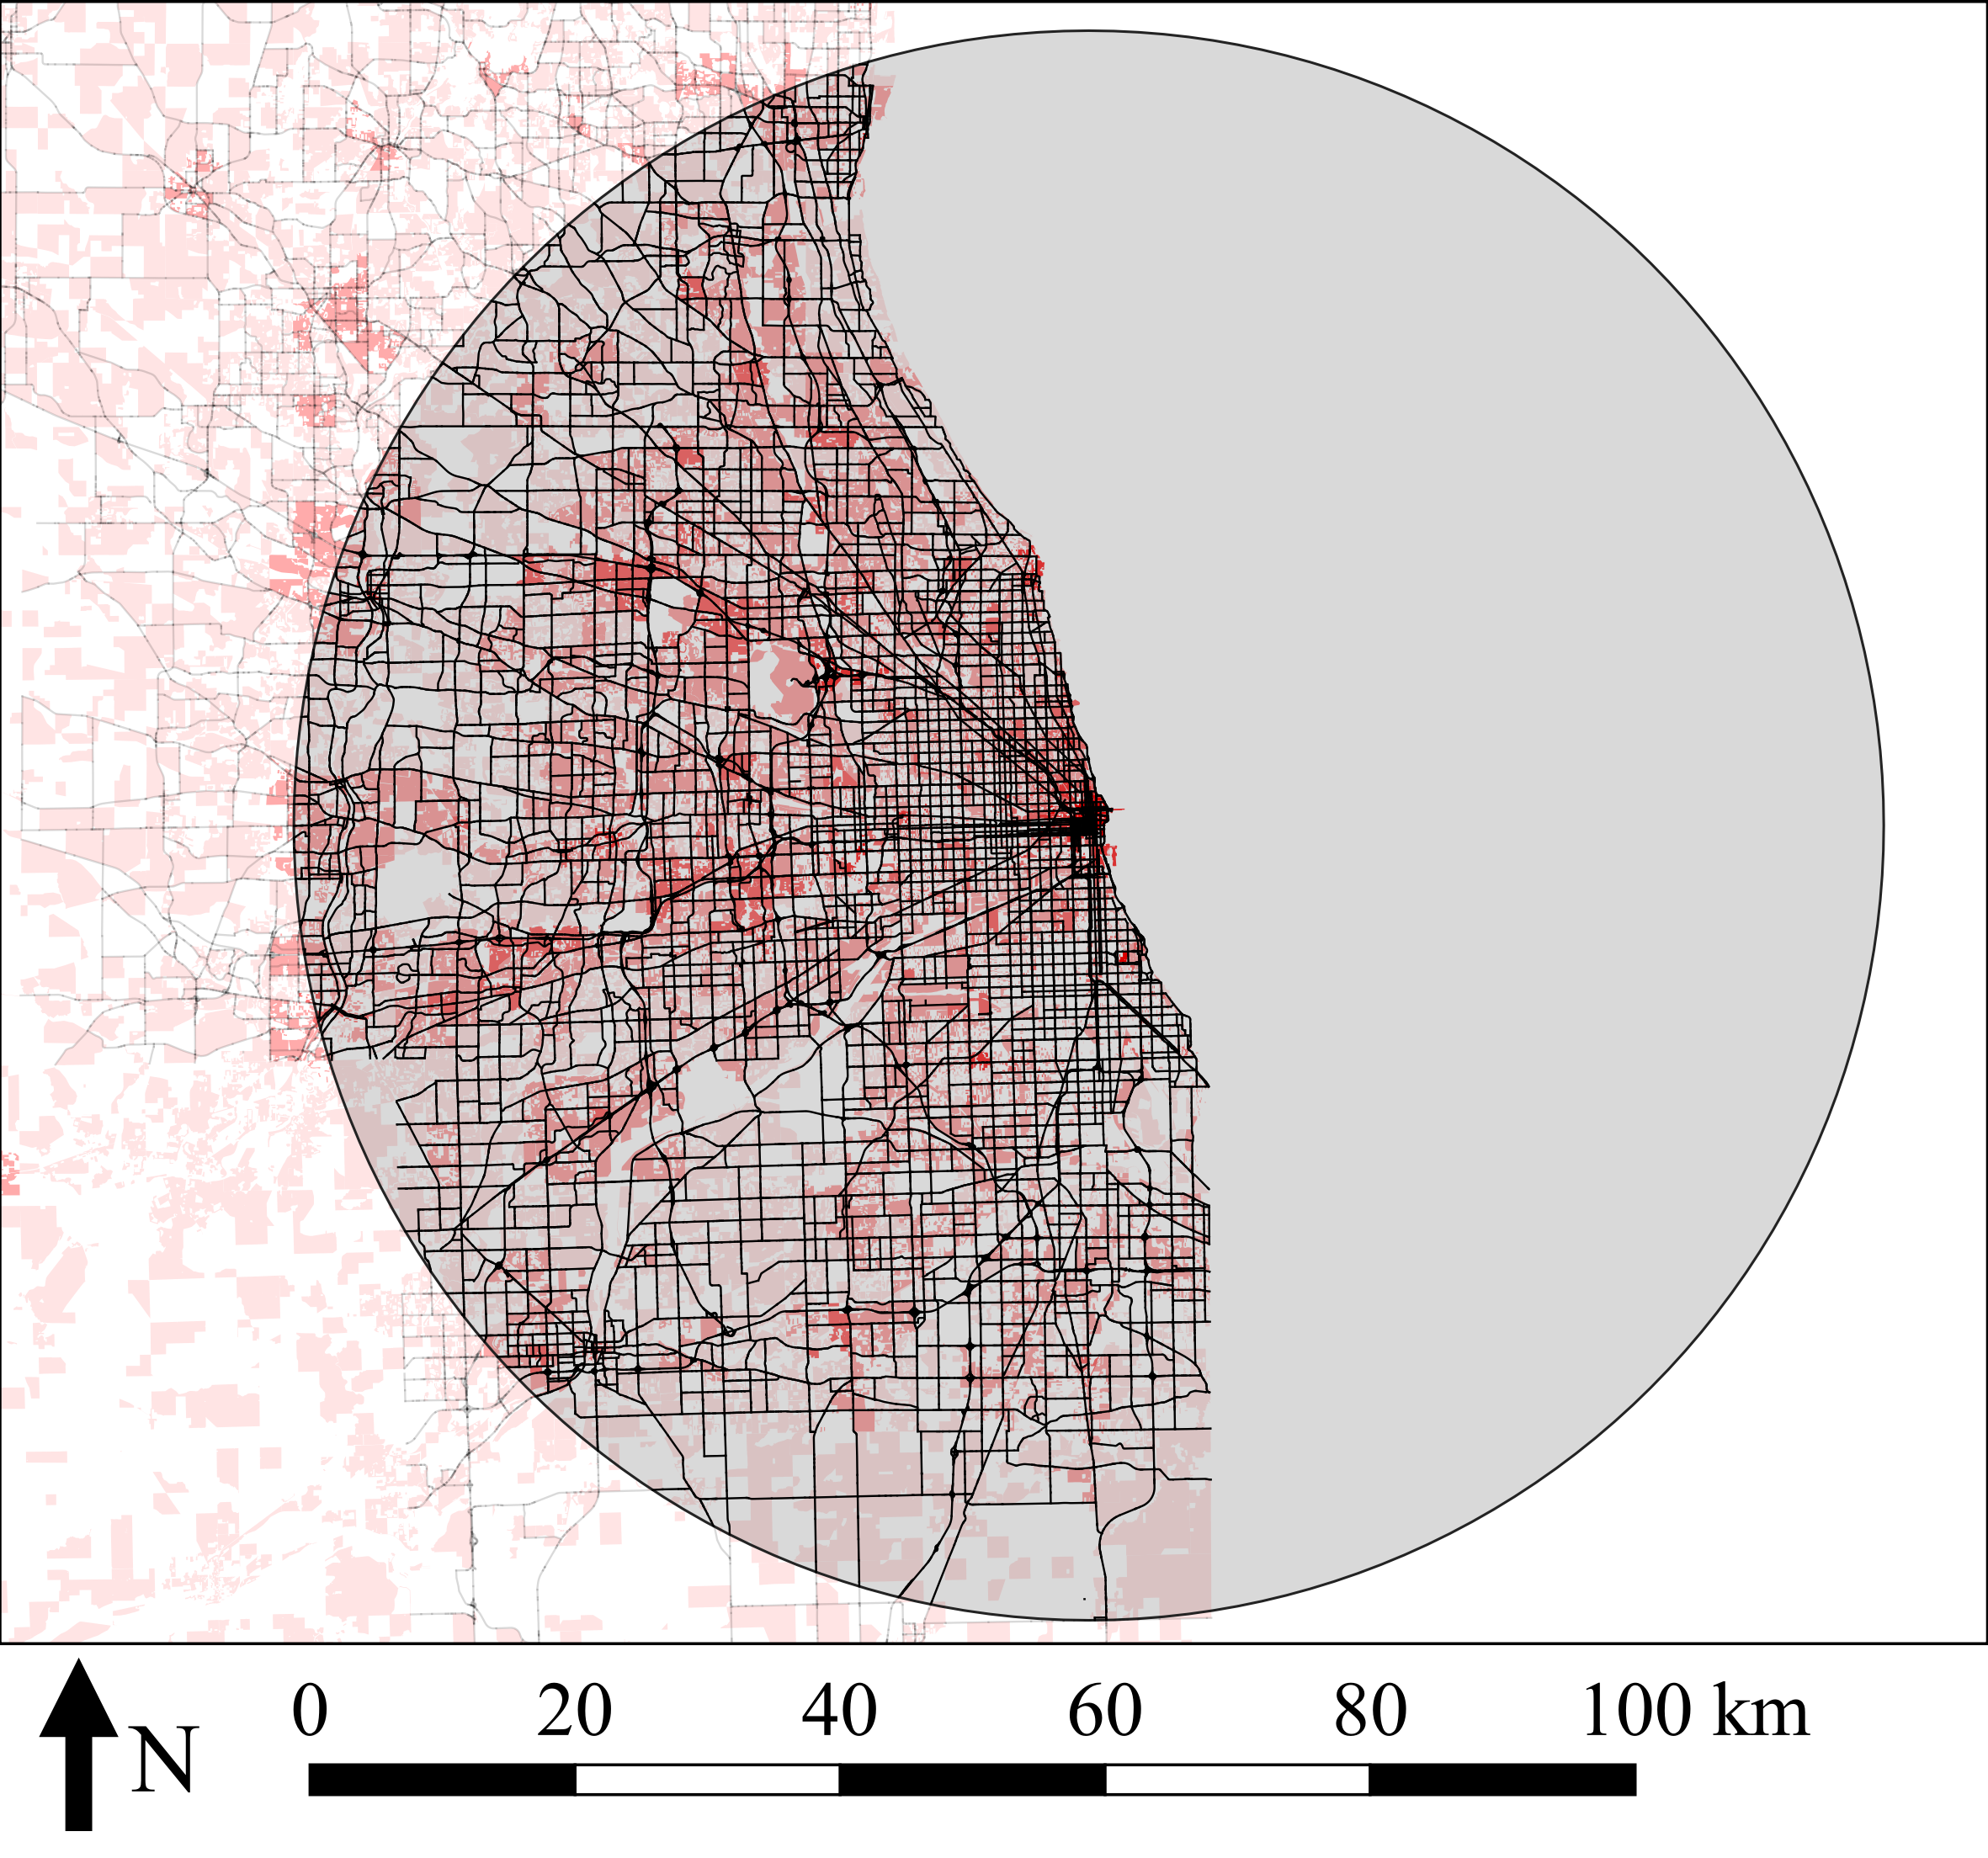
\includegraphics[width=\textwidth]{chi_vicmap}
        \caption{Chicago, IL}
         \label{fig:chimap}
     \end{subfigure}
     
	\caption{Street network and employment density in select cities}
    \label{fig:vicmap}
\end{figure}

\pagebreak

A summary of results and additional density distribution statistics are presented in Table~\ref{tab:multicityresults}. The city street networks vary due to geography and land use (e.g., proximity to agriculture, mountains, and bodies of water), but still largely maintain a fairly uniformly grid-like street network where possible. However, an interesting difference is the variation in overall employment density and the distribution of density in each city. Figure~\ref{fig:empdens} demonstrates the relative variation in employment density across the different cities. Chicago is the largest, densest city, and likely the most monocentric city of the group with the highest average density and standard deviation of density of 3,869 and 13,696 jobs per square kilometer, respectively. This is evident in Figure~\ref{fig:empdens_log}, with Chicago maintaining a relatively high density beyond where most cities begin to taper off. Fresno and Tucson possess the lowest density, which is likely proportional to their overall population, but Tucson does have a much higher standard deviation relative to its mean density, indicating there may be pockets of very high density.

\begin{figure}[H]
     \centering
     \begin{subfigure}[b]{0.49\textwidth}
         \centering
\begin{knitrout}
\definecolor{shadecolor}{rgb}{0.969, 0.969, 0.969}\color{fgcolor}
\includegraphics[width=\textwidth]{figure/empdens_log-1} 
\end{knitrout}
    \caption{Smoothed employment density distribution for different cities plotted on logarithmic scale}
    \label{fig:empdens_log}
     \end{subfigure}
     \hfill
     \begin{subfigure}[b]{0.49\textwidth}
         \centering
\begin{knitrout}
\definecolor{shadecolor}{rgb}{0.969, 0.969, 0.969}\color{fgcolor}
\includegraphics[width=\textwidth]{figure/empdens_bar-1} 
\end{knitrout}
    \caption{Average aggregated employment density distribution for different cities}
    \label{fig:empdens_bar}
     \end{subfigure}
	\caption{Distribution of employment density by distance from city center for different cities}
    \label{fig:empdens}
\end{figure}

The trip demand parameters, $\lambda_c$ and $\lambda_b$, are roughly approximated from the statistical values of employment density for each city. Baseline trip demand, $\lambda_b$, is calculated as median employment density divided by the number of daytime travel hours (15 hours from 5am to 8pm). Monocentric demand, $\lambda_c$, is calculated as the mean density divided by the coefficient of variation (i.e., ratio of mean to standard deviation) divided by number of daytime travel hours. This procedure is highly generalized and does not capture the true spatial monocentricity of trip density. Furthermore, the street network density is also roughly approximated using only the \emph{major} streets defined by local jurisdictions (e.g., arterial functional classification). This not only ignores local streets that may carry network traffic, but also does not capture any potential asymmetric network densities (e.g., road network is densest in the center and less dense at the edges). However, the procedure described is sufficient for systematically extracting basic demand parameters for demonstrating the proposed model. 


\begin{table}[H]
\centering\small
\caption{Multi-city analysis results and statistics}
\begin{tabular}{lcc ccc ccc ccc}
\toprule
 & \multicolumn{4}{ c }{Employment density statistics} & & & & & & & Avg.\\
\cline{2-5}
City & Mean & Median & Std Dev. & $n$ zones & $R$ & $\delta$ & $\lambda_c$ & $\lambda_b$ & $\gamma$ & $\tau$ & travel time \\ \hline

Chicago & 3,869 & 1,824 & 13,696 & 1,075 & 30 & 2.4 & 73 & 122 & 8.7 & 14.5 & 117 \\

Denver & 1,613 & 757 & 3,609 & 356 & 20 & 2.7 & 48 & 50 & 4.0 & 6.6 & 83 \\

Fresno & 931 & 514 & 1,325 & 154 & 20 & 2.0 & 44 & 34 & 4.2 & 7.7 & 81 \\

Las Vegas & 1,249 & 735 & 2,396 & 428 & 20 & 2.6 & 43 & 49 & 3.8 & 7.1 & 82 \\

Melbourne & 2,886 & 1,000 & 9,192 & 112 & 15 & 2.8 & 60 & 67 & 2.4 & 4.9 & 58 \\

Sacramento & 1,310 & 499 & 3,239 & 356 & 30 & 2.8 & 35 & 33 & 5.7 & 11.6 & 121 \\

Tucson & 1,086 & 424 & 2,877 & 186 & 20 & 1.8 & 27 & 28 & 2.3 & 7.7 & 71 \\\bottomrule
\end{tabular}
\label{tab:multicityresults}
\end{table}

The results shown in Table~\ref{tab:multicityresults} yields a pedestrianized zone surrounded by a transit priority zone in each city, but varying in sizes. Unsurprisingly Chicago yields the largest zones of radius 8.7 km and 14.5 km, respectively. Pedestrianization would encompass most of the inner neighborhoods, approximately halfway to Chicago Midway Airport, and transit priority to just beyond Midway Airport. While full pedestrianization at this scale is impractical, partial pedestrianization that discourages through traffic is more realistic. Transit priority is less unrealistic, with transit in this zone already being well serviced by Chicago's urban rail system. In contrast, Sacramento yielded a surprisingly large transit priority zone considering the city's low density sprawl. This may be a result of the large proportion of monocentric demand to baseline demand.

It should be strongly stated that these results very rough. However, the results do provide interesting general insight and also demonstrate the applicability of this model. It is possible that future applications could implement the model on a more localized neighborhood-scale to better suit polycentric cities. 


\section{Discussion}
While the model can be utilized for the immediate purpose of determining optimal zone sizing, traffic flow characteristics, and travel time across the city's street network; this is not necessarily practical as the model is based on an idealized city, nor is the primary purpose in this paper. The key objective is to demonstrate the complementary benefits of pedestrianized and transit priority zones in a city. However, the model presented is highly idealized. In reality most cities are incredibly complex, diverse, and asymmetric. Furthermore, the model also does not account for the multitude of social and behavioral factors that often play a critical role in transportation and urban systems. To summarize, the model possesses four critical weaknesses:

%\begin{itemize}
The model does not account for suppressed demand. Comparing the base case with the optimal case, it is clear that the pedestrianization and transit priority zones enable 100\% of demand to be served without the severe breakdown in traffic flow observed in the base case in Figure~\ref{fig:baselinett}. In reality the network would likely not reach such extreme traffic flow break down as demand would simply be suppressed, with a certain portion of demand choosing to use transit out of necessity (e.g., low income), convenience (e.g., commuter rail), or various other factors; ultimately finding some other equilibrium point. However, this is not necessarily a model flaw, but is important as this suppressed equilibrium point is sub-optimal, resulting in depressed mobility, dampened economic activity, and lacks the social and environmental benefits of a dense pedestrian oriented city center. This is a critical issue, merely managing demand through harsh travel restrictions or economic policies (e.g., road-space rationing or tolls) with no reasonable alternative serves only to suppress demand and activity. Moreover, this can also have severe equity implications by disproportionately restricting access to jobs and leisure, burdening those who cannot easily afford higher-cost road pricing or circumvent travel restrictions. This point is particularly important, considering pedestrianization is generally intended to provide a social benefit.

The model has no account for cost or pricing. This is a critical weakness, not only in terms of mode-choice modeling, but in accounting for ``softer'' economic policies, such as congestion pricing (e.g., London, Stockholm, and New York City), that are less aggressive than physical barriers and alleviate the freight and emergency services issue. This is conceptually similar in that it reduces automobile usage in a zone (albeit through economic barriers), but is important practically as it allows for a transfer of funds from one mode to another. This is especially important when considering equity impacts of exclusionary policies. However, monetary costs could be incorporated into future models by converting to temporal costs. Such a model would further benefit from a heterogeneous population of travelers in order to measure equity impacts.

The model assumes infinite transit capacity with no congestion impacts. Although transit has the potential to offer substantially higher capacity than single occupancy automobiles, limits do exist and transit service is often impacted by passenger congestion (e.g., increased dwell time from door crowding). For clarity it was assumed that transit priority offers reliable service relative to automobiles, but these considerations could be accounted for in future models. Furthermore, this model is highly generalized and assumes no impact on automobile congestion from transit priority. While this may be true for vertically separated transit right-of-ways, such as elevated tracks or subways, this may not be true for at-grade space is allocation, such as dedicated bus lanes.

The model assumes uniform pedestrianization and transit priority zoning. In reality it is possible that certain streets or partial pedestrianization can happen. This also ignores practical issues such as emergency services and freight delivery. For example, San Francisco's Market Street prohibits private automobiles, but allows delivery vehicles and taxis. There also exists a spectrum of transit priority, from transit signal priority only, to a fully separated right-of-way. Future research could address this using some priority/pedestrianization scale (e.g., from 0 to 100\%) to account for this effect, rather than a binary transit priority and pedestrianized zone.
%\end{itemize}

Despite these weaknesses, the model does offer valuable insights on pedestrianization and transit priority policies. The major finding from this analysis is the travel time benefit and network capacity gained with the optimal pedestrian and transit priority zone compared to the base case with no policy intervention (see Figure~\ref{fig:comparett}). In addition, the model also provides a potentially useful tool in determining the overall travel demand threshold where transit priority is justifiable. 

\section{Conclusion}
As countless urban planners have sought to articulate, dense walkable city centers offer a plethora of benefits. From more efficient land-use utilization with less land dedicated to roads, highways and parking; environmental gains from reduced emissions and the urbanized footprint; public health gains from active transportation (e.g., walking and biking) and improved air quality; to economic growth and resiliency by reducing congestion and unlocking potentially suppressed travel demand. The analytical model developed in this paper seeks to validate this by objectively demonstrating the potential complementary benefits to travel time with a pedestrianized zone surrounded by a transit priority zone in a city with a rectilinear street network. 

The optimal case with pedestrianized and transit priority zones not only provided a pedestrian oriented city center, meeting social objectives, but also greatly increased the network capacity of the city, satisfying the engineering and economic objectives. Overall, the analytical model reveals general insight on the complementary benefits of pedestrianized and transit priority zones in allowing greater network capacity while providing desirable pedestrian oriented urbanism. Insights from this analysis are most directly applicable to large dense cities with robust existing transit systems, but could also be used with smaller cities to approximate when pedestrianization and transit priority is, or is not, effective. Furthermore, while the model lacks several important considerations (e.g., transit capacity, non-binary zoning, pricing, and heterogeneous travelers), it firmly establishes the fundamentals that could be easily expanded in future work.

\section*{Acknowledgments}
The author would like to acknowledge Dr. Gonzales of the University of Massachusetts Amherst for the initial formulation of network traffic flow in a circular city \citep{Gonzales2015,Fournier2018a, Fournier2019}, from which this model was originally conceived.

% \printbibliography
% \bibliographystyle{agsm}
\bibliography{references.bib}

\end{document}
